%-----------------------------------------------------------------------
%                                                                 aa.tex
% AA vers. 9.4, LaTeX class for Astronomy & Astrophysics
% Demonstration file
%                                                       (c) EDP Sciences
%-----------------------------------------------------------------------
%
%\documentclass[referee]{aa}    % for a referee version
%\documentclass[onecolumn]{aa}  % for a paper on 1 column  
%\documentclass[longauth]{aa}   % for long lists of authors and/or affiliations. 
                                % This command displays the first eight authors on page 1
                                % and shift the whole list after the references.
                                % Ensure to separate each author with the \and command (see below)
%\documentclass[letter]{aa}     % for the letters
%\documentclass[bibyear]{aa}    % if the references are not structured
                                % according to the author-year natbib style

\documentclass{aa}  

\usepackage{graphicx}
\usepackage{txfonts}
\usepackage{lipsum}
\usepackage{subcaption}         % necessary for continued figures, example in section 3
                                % and appendix
\usepackage{lscape}             % to rotate a single page table, example in appendix.
                                % For landscape tables, see the longtable examples.
\usepackage{placeins}           % useful with \FloatBarrier, to keep 
                                % onecolumn floats from drifting to the next section
                                
%%%%%%%%%%%%%%%%%%%%%%%%%%%%%%%%%%%%%%%%
%\usepackage[options]{hyperref}
% To add links in your PDF file, use the package "hyperref"
% with options according to your LaTeX or PDFLaTeX drivers.
%%%%%%%%%%%%%%%%%%%%%%%%%%%%%%%%%%%%%%%%

\begin{document}

%%%%%%%%%%%%%%%%%%%%%%%%%%%%%%%%%%%%%%%%
% if you use custom commands in your title,
% ensure to check your title when submitting!
%%%%%%%%%%%%%%%%%%%%%%%%%%%%%%%%%%%%%%%%
   \title{Astronomy \& Astrophysics \LaTeX\ template}


%%%%%%%%%%%%%%%%%%%%%%%%%%%%%%%%%%%%%%%%
% Please separate each author with the \and command
%
% Use the \corrauth to provide the corresponding
% author address. It will be automatically inserted as 
% footnote in the PDF output.
%
% Please DO NOT include ORCIDs next to author names.
% Instead, please provide an active address for each coauthor:
% it will be automatically extracted by EDPS editorial system, 
% and co-authors will be be able to authenticate their ORCID.
%
% Only authenticated ORCIDs will be taken into account.
% ORCIDs included here will be removed.
%%%%%%%%%%%%%%%%%%%%%%%%%%%%%%%%%%%%%%%%

   \author{Xavier Garcia Sàbat\inst{1}\corrauth{xavier.garcia@uib.cat}        % use \corrauth for the corresponding author
        \and David Keitel\inst{1}
        }

   \institute{IAC3-UIB, Universitat de les Illes Balears, Cra. de Valldemossa km 7.5. 07122 Palma, Spain}

   \date{Received September 30, 20XX}

% \abstract{}{}{}{}{}
% 5 {} token are mandatory
 
  \abstract
  % context heading (optional)
  % {} leave it empty if necessary  
   {Optional, leave empty if necessary.  The heading “Context” is used when needed to
give background information on the research conducted in the paper}
  % aims heading (mandatory)
   {Mandatory. The objectives of the paper are defined here.} 
  % methods heading (mandatory)
   {Mandatory. The methods of the investigation are outlined here}
  % results heading (mandatory)
   {Mandatory. The results are summarized here.}
  % conclusions heading (optional), leave it empty if necessary
   {Optional, leave empty if necessary.  “Conclusions” can be used to
explicit the general conclusions that can be drawn from the paper.}

   \keywords{gravitational waves -- strong gravitational lensing -- parameter estimation -- sky localization --
binary black holes -- LIGO
               }

   \maketitle



%%%%%%%%%%%%%%%%%%%%%%%%%%%%%%%%%%%%%%%%%%%%%%%%%%%%%%%%%%%%%%
\section{Introduction}
\lipsum[1]
%%%%%%%%%%%%%%%%%%%%%%%%%%%%%%%%%%%%%%%%%%%%%%%%%%%%%%%%%%%%%%
\section{Citations and maths examples}

   In this section the one-zone model of \citet{baker},
   originally used to study the Cephe{\"{\i}}d pulsation mechanism, will
   be briefly reviewed, see Fig.~\ref{fig1}, Table~\ref{t7} and Eq. (\ref{eq3}).
   For the one-zone-model Baker obtains necessary conditions
   for dynamical, secular and vibrational (or pulsational)
   stability (Eqs.\ (34a,\,b,\,c) in Baker \citeyear{baker}).
   
   \begin{equation}
    \label{eq1}
      \tau_{\mathrm{co}} = \frac{E_{\mathrm{th}}}{L_{r0}} \,,
   \end{equation}
   and the \emph{local free-fall time}
   \begin{equation}
      \tau_{\mathrm{ff}} =
         \sqrt{ \frac{3 \pi}{32 G} \frac{4\pi r_0^3}{3 M_{\mathrm{r}}}
}\,,
   \end{equation}
   Baker's $K$ and $\sigma_0$ have the following form:
   \begin{eqnarray}
   \label{eq3}
      \sigma_0 & = & \frac{\pi}{\sqrt{8}}
                     \frac{1}{ \tau_{\mathrm{ff}}} \\
      K        & = & \frac{\sqrt{32}}{\pi} \frac{1}{\delta}
                        \frac{ \tau_{\mathrm{ff}} }
                             { \tau_{\mathrm{co}} }\,;
   \end{eqnarray}
   where $ E_{\mathrm{th}} \approx m (P_0/{\rho_0})$ has been used and
   \begin{equation}
   \begin{array}{l}
      \delta = - \left(
                    \frac{ \partial \ln \rho }{ \partial \ln T }
                 \right)_P \\
      e=mc^2
   \end{array}
   \end{equation}
   is a thermodynamical quantity which is of order $1$ and equal to $1$
   for nonreacting mixtures of classical perfect gases. The physical
   meaning of $ \sigma_0 $ and $K$ is clearly visible in the equations
   above. $\sigma_0$ represents a frequency of the order one per
   free-fall time. $K$ is proportional to the ratio of the free-fall
   time and the cooling time. Substituting into Baker's criteria, using
   thermodynamic identities and definitions of thermodynamic quantities,
   \begin{displaymath}
      \Gamma_1      = \left( \frac{ \partial \ln P}{ \partial\ln \rho}
                           \right)_{S}    \, , \;
      \chi^{}_\rho  = \left( \frac{ \partial \ln P}{ \partial\ln \rho}
                           \right)_{T}    \, , \;
      \kappa^{}_{P} = \left( \frac{ \partial \ln \kappa}{ \partial\ln P}
                           \right)_{T}
   \end{displaymath}
   \begin{displaymath}
      \nabla_{\mathrm{ad}} = \left( \frac{ \partial \ln T}
                             { \partial\ln P} \right)_{S} \, , \;
      \chi^{}_T       = \left( \frac{ \partial \ln P}
                             { \partial\ln T} \right)_{\rho} \, , \;
      \kappa^{}_{T}   = \left( \frac{ \partial \ln \kappa}
                             { \partial\ln T} \right)_{T}
   \end{displaymath}



%_____________________________________________________________
%                     Onecolumn continued float (place early!)
%-------------------------------------------------------------
   \begin{figure*}
        \centering
        
\includegraphics{figure.eps}
        
\includegraphics[angle=90]{figure.eps}
        
\includegraphics{figure.eps}
        {\caption{A onecolumn \textbackslash figure* with six graphics}}
        \ContinuedFloat %      \usepackage{subcaption}
        
\includegraphics[angle=90]{figure.eps}
        
\includegraphics{figure.eps}
        
\includegraphics[angle=90]{figure.eps}
        \caption{continued.}
        \label{FigGam}%
    \end{figure*}

% %_____________________________________________________________
% %                      Another onecolumn float (place early!)
% %-------------------------------------------------------------
% \begin{figure*}[ht!]
%    \resizebox{\hsize}{!}
%             {
\includegraphics {figure.eps}}
%             %{
\includegraphics[bb=10 20 100 100,clip]{figure.eps}}
%       \caption{Another onecolumn figure*}
%          \label{wide}
% \end{figure*}
% \twocolumn
% \clearpage
% % %%%%%%%%%%%%%%%%%%%%%%%%%%%%%%%%%%%%%%%%%%%%%%%%%%%%%%%%%%%%%%


\section{Figures examples}
Examples of figures using graphicx. 
The guide "Using Imported Graphics in LaTeX2e" by Keith Reckdahl
is available on a lot of \LaTeX public servers or CTAN mirrors.


%_____________________________________________________________
%                        A figure as large as the column width
%-------------------------------------------------------------
   \begin{figure}[ht!]
   \centering
   
\includegraphics[width=\hsize]{figure.eps}
      \caption{Figure as large as the column width}
         \label{fig1}
   \end{figure}
%
%_____________________________________________________________
%                                             A rotated figure
%-------------------------------------------------------------
   \begin{figure}[ht!]
   \centering
   
\includegraphics[angle=-90,width=2cm]{figure.eps}
      \caption{Rotated figure}
         \label{fig2}
   \end{figure}
%
%_____________________________________________________________
%                        Figure with caption on the right side
%-------------------------------------------------------------
   \begin{figure}[ht!]
   \sidecaption
   
\includegraphics[width=2cm]{figure.eps}
      \caption{Figure with caption on the right side}
         \label{fig3}
   \end{figure}


%_____________________________________________________________
%                                Figure with a new BoundingBox
%-------------------------------------------------------------
   \begin{figure}
   \centering
   
\includegraphics[bb=5 20 60 60,width=3cm,clip]{figure.eps}
      \caption{Figure with a new BoundingBox}
         \label{fig4}
   \end{figure}



%_____________________________________________________________
%                              A figure including two graphics
%-------------------------------------------------------------
   \begin{figure}[ht!]
   \centering
    
\includegraphics{figure.eps}
    
\includegraphics[angle=90]{figure.eps}
    
\includegraphics{figure.eps}
      \caption{A figure including three graphics}
         \label{fig5}
   \end{figure}


%_____________________________________________________________
%                                   Continued figure numbering
%      \usepackage{subcaption} and the command \ContinuedFloat
%-------------------------------------------------------------

    \begin{figure}
    \centering
    
\includegraphics[width=3cm]{figure.eps}
      \caption{Continued figure numbering}
         \label{cont1}
    
    \centering
    \ContinuedFloat %      \usepackage{subcaption}
    
\includegraphics[width=3cm]{figure.eps}
        \caption{continued.}
             \label{cont2}

    \centering
    \ContinuedFloat %      \usepackage{subcaption}
    
\includegraphics[width=3cm]{figure.eps}
        \caption{continued.}
             \label{cont3}
    \end{figure}


\clearpage

%%%%%%%%%%%%%%%%%%%%%%%%%%%%%%%%%%%%%%%%%%%%%%%%%%%%%%%%%%%%%%
\section{Tables examples}



The jump in table numbering below is caused by the command
\textbackslash longtable*. This command only works in the onecolumn
environment. For this reason, we recommend either:
\begin{itemize}
\item placing your long tables in onecolumn appendices (cf.~\ref{ltapp} and ~\ref{lsltapp}),
\item or using the longtab environment as illustrated by tables ~\ref{longtable1} and ~\ref{longtable2}.
Note that the longtab environment will preserve the table
numbering and automatically places long tables after the appendices.
They will be moved inside the appendices by the Publisher, if necessary.
\end{itemize}

%_____________________________________________________________
%                                             Simple A&A Table
%-------------------------------------------------------------
\begin{table}[ht!]
\caption{Simple A\&A Table}                 % title of Table
\label{table:1}    % is used to refer this table in the text
\centering                        % used for centering table
\begin{tabular}{c c c c}      % centered columns (4 columns)
\hline\hline               % inserts double horizontal lines
HJD & $E$ & Method\#2 & Method\#3 \\         % table heading
\hline                      % inserts single horizontal line
   1 & 50 & $-837$ & 970 \\    % inserting body of the table
   2 & 47 & 877    & 230 \\
\hline                                  %inserts single line
\end{tabular}
\end{table}


%%%%%%%%%%%%%%%%%%%%%%%%%%%%%%%%%%%%%%%%%%%%%%%%%%%%%%%%%%%%%%%
%                                                  Long tables
%%%%%%%%%%%%%%%%%%%%%%%%%%%%%%%%%%%%%%%%%%%%%%%%%%%%%%%%%%%%%%%
%_____________________________________________________________
%                     Long table using the longtab environment
%-------------------------------------------------------------
\longtab[1]{
\begin{longtable}{lllrrr}
\caption{A long table using the longtab environment}\\
\label{longtable1}\\
\hline\hline
Catalogue& $M_{V}$ & Spectral & Distance & Mode & Count Rate \\
\hline
\endfirsthead
\caption{continued.}\\
\hline\hline
Catalogue& $M_{V}$ & Spectral & Distance & Mode & Count Rate \\
\hline
\endhead
\hline
\endfoot
%%
Gl 33    & 6.37 & K2 V & 7.46 & S & 0.043170\\
Gl 66AB  & 6.26 & K2 V & 8.15 & S & 0.260478\\
Gl 68    & 5.87 & K1 V & 7.47 & P & 0.026610\\
         &      &      &      & H & 0.008686\\
Gl 86
\footnote{Source not included in the HRI catalog. See Sect.~5.4.2 for details.}
         & 5.92 & K0 V & 10.91& S & 0.058230\\
                  & 5.92 & K0 V & 10.91& S & 0.058230\\
Gl 33    & 6.37 & K2 V & 7.46 & S & 0.043170\\
Gl 66AB  & 6.26 & K2 V & 8.15 & S & 0.260478\\
Gl 68    & 5.87 & K1 V & 7.47 & P & 0.026610\\
         &      &      &      & H & 0.008686\\
Gl 86    & 5.92 & K0 V & 10.91& S & 0.058230\\            & 5.92 & K0 V & 10.91& S & 0.058230\\
Gl 33    & 6.37 & K2 V & 7.46 & S & 0.043170\\
Gl 66AB  & 6.26 & K2 V & 8.15 & S & 0.260478\\
Gl 68    & 5.87 & K1 V & 7.47 & P & 0.026610\\
         &      &      &      & H & 0.008686\\
Gl 86    & 5.92 & K0 V & 10.91& S & 0.058230\\            & 5.92 & K0 V & 10.91& S & 0.058230\\
Gl 33    & 6.37 & K2 V & 7.46 & S & 0.043170\\
Gl 66AB  & 6.26 & K2 V & 8.15 & S & 0.260478\\
Gl 68    & 5.87 & K1 V & 7.47 & P & 0.026610\\
         &      &      &      & H & 0.008686\\
Gl 86    & 5.92 & K0 V & 10.91& S & 0.058230\\            & 5.92 & K0 V & 10.91& S & 0.058230\\
Gl 33    & 6.37 & K2 V & 7.46 & S & 0.043170\\
Gl 66AB  & 6.26 & K2 V & 8.15 & S & 0.260478\\
Gl 68    & 5.87 & K1 V & 7.47 & P & 0.026610\\
         &      &      &      & H & 0.008686\\
Gl 86    & 5.92 & K0 V & 10.91& S & 0.058230\\            & 5.92 & K0 V & 10.91& S & 0.058230\\
Gl 33    & 6.37 & K2 V & 7.46 & S & 0.043170\\
Gl 66AB  & 6.26 & K2 V & 8.15 & S & 0.260478\\
Gl 68    & 5.87 & K1 V & 7.47 & P & 0.026610\\
         &      &      &      & H & 0.008686\\
Gl 86    & 5.92 & K0 V & 10.91& S & 0.058230\\            & 5.92 & K0 V & 10.91& S & 0.058230\\
Gl 33    & 6.37 & K2 V & 7.46 & S & 0.043170\\
Gl 66AB  & 6.26 & K2 V & 8.15 & S & 0.260478\\
Gl 68    & 5.87 & K1 V & 7.47 & P & 0.026610\\
         &      &      &      & H & 0.008686\\
Gl 86    & 5.92 & K0 V & 10.91& S & 0.058230\\            & 5.92 & K0 V & 10.91& S & 0.058230\\
Gl 33    & 6.37 & K2 V & 7.46 & S & 0.043170\\
Gl 66AB  & 6.26 & K2 V & 8.15 & S & 0.260478\\
Gl 68    & 5.87 & K1 V & 7.47 & P & 0.026610\\
         &      &      &      & H & 0.008686\\
Gl 86    & 5.92 & K0 V & 10.91& S & 0.058230\\            & 5.92 & K0 V & 10.91& S & 0.058230\\
Gl 33    & 6.37 & K2 V & 7.46 & S & 0.043170\\
Gl 66AB  & 6.26 & K2 V & 8.15 & S & 0.260478\\
Gl 68    & 5.87 & K1 V & 7.47 & P & 0.026610\\
         &      &      &      & H & 0.008686\\
Gl 86    & 5.92 & K0 V & 10.91& S & 0.058230\\            & 5.92 & K0 V & 10.91& S & 0.058230\\
Gl 33    & 6.37 & K2 V & 7.46 & S & 0.043170\\
Gl 66AB  & 6.26 & K2 V & 8.15 & S & 0.260478\\
Gl 68    & 5.87 & K1 V & 7.47 & P & 0.026610\\
         &      &      &      & H & 0.008686\\
Gl 86    & 5.92 & K0 V & 10.91& S & 0.058230\\
         & 5.92 & K0 V & 10.91& S & 0.058230\\
Gl 33    & 6.37 & K2 V & 7.46 & S & 0.043170\\
Gl 66AB  & 6.26 & K2 V & 8.15 & S & 0.260478\\
Gl 68    & 5.87 & K1 V & 7.47 & P & 0.026610\\
         &      &      &      & H & 0.008686\\
Gl 86    & 5.92 & K0 V & 10.91& S & 0.058230\\            & 5.92 & K0 V & 10.91& S & 0.058230\\
Gl 33    & 6.37 & K2 V & 7.46 & S & 0.043170\\
Gl 66AB  & 6.26 & K2 V & 8.15 & S & 0.260478\\
Gl 68    & 5.87 & K1 V & 7.47 & P & 0.026610\\
         &      &      &      & H & 0.008686\\
Gl 86    & 5.92 & K0 V & 10.91& S & 0.058230\\
         & 5.92 & K0 V & 10.91& S & 0.058230\\
Gl 33    & 6.37 & K2 V & 7.46 & S & 0.043170\\
Gl 66AB  & 6.26 & K2 V & 8.15 & S & 0.260478\\
Gl 68    & 5.87 & K1 V & 7.47 & P & 0.026610\\
         &      &      &      & H & 0.008686\\
Gl 86    & 5.92 & K0 V & 10.91& S & 0.058230\\            & 5.92 & K0 V & 10.91& S & 0.058230\\
Gl 33    & 6.37 & K2 V & 7.46 & S & 0.043170\\
Gl 66AB  & 6.26 & K2 V & 8.15 & S & 0.260478\\
Gl 68    & 5.87 & K1 V & 7.47 & P & 0.026610\\
         &      &      &      & H & 0.008686\\
Gl 86    & 5.92 & K0 V & 10.91& S & 0.058230\\            & 5.92 & K0 V & 10.91& S & 0.058230\\
Gl 33    & 6.37 & K2 V & 7.46 & S & 0.043170\\
Gl 66AB  & 6.26 & K2 V & 8.15 & S & 0.260478\\
Gl 68    & 5.87 & K1 V & 7.47 & P & 0.026610\\
         &      &      &      & H & 0.008686\\
Gl 86    & 5.92 & K0 V & 10.91& S & 0.058230\\            & 5.92 & K0 V & 10.91& S & 0.058230\\
Gl 33    & 6.37 & K2 V & 7.46 & S & 0.043170\\
Gl 66AB  & 6.26 & K2 V & 8.15 & S & 0.260478\\
Gl 68    & 5.87 & K1 V & 7.47 & P & 0.026610\\
         &      &      &      & H & 0.008686\\
Gl 86    & 5.92 & K0 V & 10.91& S & 0.058230\\   
\end{longtable}
}


%_____________________________________________________________
%       Long table in landscape using the longtab environment
%-------------------------------------------------------------
\longtab[2]{
\begin{landscape}
\begin{longtable}{lllrrr}
\caption{A long landscape table using the longtab environment}\\
\label{longtable2} \\
\hline\hline
Catalogue& $M_{V}$ & Spectral & Distance & Mode & Count Rate \\
\hline
\endfirsthead
\caption{continued.}\\
\hline\hline
Catalogue& $M_{V}$ & Spectral & Distance & Mode & Count Rate \\
\hline
\endhead
\hline
\endfoot
%%
Gl 33    & 6.37 & K2 V & 7.46 & S & 0.043170\\
Gl 66AB  & 6.26 & K2 V & 8.15 & S & 0.260478\\
Gl 68    & 5.87 & K1 V & 7.47 & P & 0.026610\\
         &      &      &      & H & 0.008686\\
Gl 86
\footnote{Source not included in the HRI catalog. See Sect.~5.4.2 for details.}
         & 5.92 & K0 V & 10.91& S & 0.058230\\
         Gl 33    & 6.37 & K2 V & 7.46 & S & 0.043170\\
Gl 66AB  & 6.26 & K2 V & 8.15 & S & 0.260478\\
Gl 68    & 5.87 & K1 V & 7.47 & P & 0.026610\\
         &      &      &      & H & 0.008686\\
Gl 86    & 5.92 & K0 V & 10.91& S & 0.058230\\
Gl 33    & 6.37 & K2 V & 7.46 & S & 0.043170\\
Gl 66AB  & 6.26 & K2 V & 8.15 & S & 0.260478\\
Gl 68    & 5.87 & K1 V & 7.47 & P & 0.026610\\
         &      &      &      & H & 0.008686\\
Gl 86    & 5.92 & K0 V & 10.91& S & 0.058230\\   Gl 33    & 6.37 & K2 V & 7.46 & S & 0.043170\\
Gl 66AB  & 6.26 & K2 V & 8.15 & S & 0.260478\\
Gl 68    & 5.87 & K1 V & 7.47 & P & 0.026610\\
         &      &      &      & H & 0.008686\\
Gl 86    & 5.92 & K0 V & 10.91& S & 0.058230\\   Gl 33    & 6.37 & K2 V & 7.46 & S & 0.043170\\
Gl 66AB  & 6.26 & K2 V & 8.15 & S & 0.260478\\
Gl 68    & 5.87 & K1 V & 7.47 & P & 0.026610\\
         &      &      &      & H & 0.008686\\
Gl 86    & 5.92 & K0 V & 10.91& S & 0.058230\\   Gl 33    & 6.37 & K2 V & 7.46 & S & 0.043170\\
Gl 66AB  & 6.26 & K2 V & 8.15 & S & 0.260478\\
Gl 68    & 5.87 & K1 V & 7.47 & P & 0.026610\\
         &      &      &      & H & 0.008686\\
Gl 86    & 5.92 & K0 V & 10.91& S & 0.058230\\   Gl 33    & 6.37 & K2 V & 7.46 & S & 0.043170\\
Gl 66AB  & 6.26 & K2 V & 8.15 & S & 0.260478\\
Gl 68    & 5.87 & K1 V & 7.47 & P & 0.026610\\
         &      &      &      & H & 0.008686\\
Gl 86    & 5.92 & K0 V & 10.91& S & 0.058230\\   Gl 33    & 6.37 & K2 V & 7.46 & S & 0.043170\\
Gl 66AB  & 6.26 & K2 V & 8.15 & S & 0.260478\\
Gl 68    & 5.87 & K1 V & 7.47 & P & 0.026610\\
         &      &      &      & H & 0.008686\\
Gl 86    & 5.92 & K0 V & 10.91& S & 0.058230\\   Gl 33    & 6.37 & K2 V & 7.46 & S & 0.043170\\
Gl 66AB  & 6.26 & K2 V & 8.15 & S & 0.260478\\
Gl 68    & 5.87 & K1 V & 7.47 & P & 0.026610\\
         &      &      &      & H & 0.008686\\
Gl 86    & 5.92 & K0 V & 10.91& S & 0.058230\\   Gl 33    & 6.37 & K2 V & 7.46 & S & 0.043170\\
Gl 66AB  & 6.26 & K2 V & 8.15 & S & 0.260478\\
Gl 68    & 5.87 & K1 V & 7.47 & P & 0.026610\\
         &      &      &      & H & 0.008686\\
Gl 86    & 5.92 & K0 V & 10.91& S & 0.058230\\   Gl 33    & 6.37 & K2 V & 7.46 & S & 0.043170\\
Gl 66AB  & 6.26 & K2 V & 8.15 & S & 0.260478\\
Gl 68    & 5.87 & K1 V & 7.47 & P & 0.026610\\
         &      &      &      & H & 0.008686\\
Gl 86    & 5.92 & K0 V & 10.91& S & 0.058230\\   Gl 33    & 6.37 & K2 V & 7.46 & S & 0.043170\\
Gl 66AB  & 6.26 & K2 V & 8.15 & S & 0.260478\\
Gl 68    & 5.87 & K1 V & 7.47 & P & 0.026610\\
         &      &      &      & H & 0.008686\\
Gl 86    & 5.92 & K0 V & 10.91& S & 0.058230\\   Gl 33    & 6.37 & K2 V & 7.46 & S & 0.043170\\
Gl 66AB  & 6.26 & K2 V & 8.15 & S & 0.260478\\
Gl 68    & 5.87 & K1 V & 7.47 & P & 0.026610\\
         &      &      &      & H & 0.008686\\
Gl 86    & 5.92 & K0 V & 10.91& S & 0.058230\\   Gl 33    & 6.37 & K2 V & 7.46 & S & 0.043170\\
Gl 66AB  & 6.26 & K2 V & 8.15 & S & 0.260478\\
Gl 68    & 5.87 & K1 V & 7.47 & P & 0.026610\\
         &      &      &      & H & 0.008686\\
Gl 86    & 5.92 & K0 V & 10.91& S & 0.058230\\   
\end{longtable}
\end{landscape}
}
%%%%%%%%%%%%%%%%%%%%%%%%%%%%%%%%%%%%%%%%%%%%%%%%%%%%%%%%%%%%%%%
%                                           End of long tables.
%%%%%%%%%%%%%%%%%%%%%%%%%%%%%%%%%%%%%%%%%%%%%%%%%%%%%%%%%%%%%%%


%_____________________________________________________________
%                                             Table with notes
%-------------------------------------------------------------
% Single note
%-------------------------------------------------------------
\begin{table}[ht!]
\caption{\label{t7}Table with notes}
\centering
\begin{tabular}{lcc}
\hline\hline
Star&Spectral type&RA(J2000)\\
\hline
69           &B1\,V     &09 15 54.046\\
LS~1267~(86) &O8\,V     &09 15 52.787\\
24.6         &7.58      &1.37\\
\hline
MO 2-119     &B0.5\,V   &09 15 33.7\\
LS~1269      &O8.5\,V   &09 15 56.60\\
\hline
\end{tabular}
\tablefoot{The top panel shows likely members of Pismis~11. The bottom panel displays stars outside the clusters.}
\end{table}

%-------------------------------------------------------------
% More notes
%-------------------------------------------------------------
\begin{table}[ht!]
\caption{\label{t8}Table with multiple notes}
\centering
\begin{tabular}{lcc}
\hline\hline
Star&Spectral type&RA(J2000)\\
\hline
69           &B1\,V     &09 15 54.046\\
LS~1267~(86) &O8\,V     &11.07\tablefootmark{a}\\
24.6         &7.58\tablefootmark{1}&1.37\tablefootmark{a}\\
\hline
MO 2-119     &B0.5\,V   &11.74\tablefootmark{c}\\
LS~1269      &O8.5\,V   &10.85\tablefootmark{d}\\
\hline
\end{tabular}
\tablefoot{The top panel shows likely members of Pismis~11. The bottom panel displays stars outside the clusters.\\
\tablefoottext{a}{Photometry for MF13, LS~1267 and HD~80077 from
Dupont et al.}
\tablefoottext{b}{Photometry for LS~1262, LS~1269 from
Durand et al.}
\tablefoottext{c}{Photometry for MO2-119 from
Mathieu et al.}
}
\end{table}


%____________________________________________________________
%                                       Table with references
%-------------------------------------------------------------

\begin{table}[ht]
 \caption[]{\label{nearbylistaa2}Table with references}
\begin{tabular}{lccc}
 \hline \hline
 SN name&Epoch&Bands\\
 &
  (with respect to $B$ maximum) &
 &
 \\ \hline
1981B   & 0 & {\it UBV}\\
1990N   & 2, 7 & {\it UBVRI}\\
1991M   & 3 & {\it VRI}\\
\hline
\noalign{\smallskip}
\multicolumn{4}{c}{ SNe 91bg-like} \\
\noalign{\smallskip}
\hline
1991bg   & 1, 2 & {\it BVRI}\\
1999by   & $-$5, $-$4, $-$3, 3, 4, 5 & {\it UBVRI}\\
\hline
\noalign{\smallskip}
\multicolumn{4}{c}{ SNe 91T-like} \\
\noalign{\smallskip}
\hline
1991T   & $-$3, 0 & {\it UBVRI}\\
2000cx  & $-$3, $-$2, 0, 1, 5 & {\it UBVRI}\\ %
\hline
\end{tabular}
\tablebib{(1)~\citet{zheng};
(2) \citet{mizuno}; (3) \citet{balluch}; (4) \citet{cox};
(5) \citet{cox69}; (6) \citet{tscharnuter}; (7) \citet{terlevich};
(8) \citet{yorke80a}.
}
\end{table}

\newpage 



\section{Results: sky localization with H1+L1}
\label{sec:results_hl}

We now assess the improvement in sky localization achieved by the coherent joint analysis of strongly lensed image pairs, relative to the analysis of each image in isolation, for the two-detector H1+L1 (HL) network under projected O5a sensitivity, across the full sample of 157 successfully analyzed events

\subsection{90\% credible sky area}
\label{sec:results_area90}

For each of the 157 events, we compute the 90\% credible sky area $A_{90}$
(Eq.~\eqref{eq:A90}) from the single-image posteriors of image~1 and
image~2, and from the joint posterior. We define the best single-image area
as $A_{90}^{\rm best} \equiv \min(A_{90}^{(1)}, A_{90}^{(2)})$, and the
per-event improvement factor from combining the two images as
\begin{equation}
    \mathrm{IF}_{\rm joint} \equiv A_{90}^{\rm best} / A_{90}^{\rm joint} .
    \label{eq:if_joint}
\end{equation}

Figure~\ref{fig:cdf_pdf_area90} shows the cumulative and probability density
distributions of $A_{90}$ for the best single-image and joint analyses. The
joint distribution is shifted to smaller areas across the entire sample: the
median 90\% credible area drops from $562.5\,\mathrm{deg}^2$ (best single
image) to $90.7\,\mathrm{deg}^2$ (joint), a median improvement factor of
$\mathrm{IF}_{\rm joint} = 5.19$. The improvement is universal, with
$\mathrm{IF}_{\rm joint} > 1$ for all 157 events (range $1.11$--$27.90$),
confirming that the gain is systematic rather than driven by a handful of
favorably placed sources. Six events ($3.8\,\%$) reach a joint area below
$10\,\mathrm{deg}^2$, the benchmark commonly adopted for host-galaxy
identification and multimessenger follow-up with wide-field survey
telescopes \citep{abbott2020prospects}.

\begin{figure}[htbp]
    \centering
    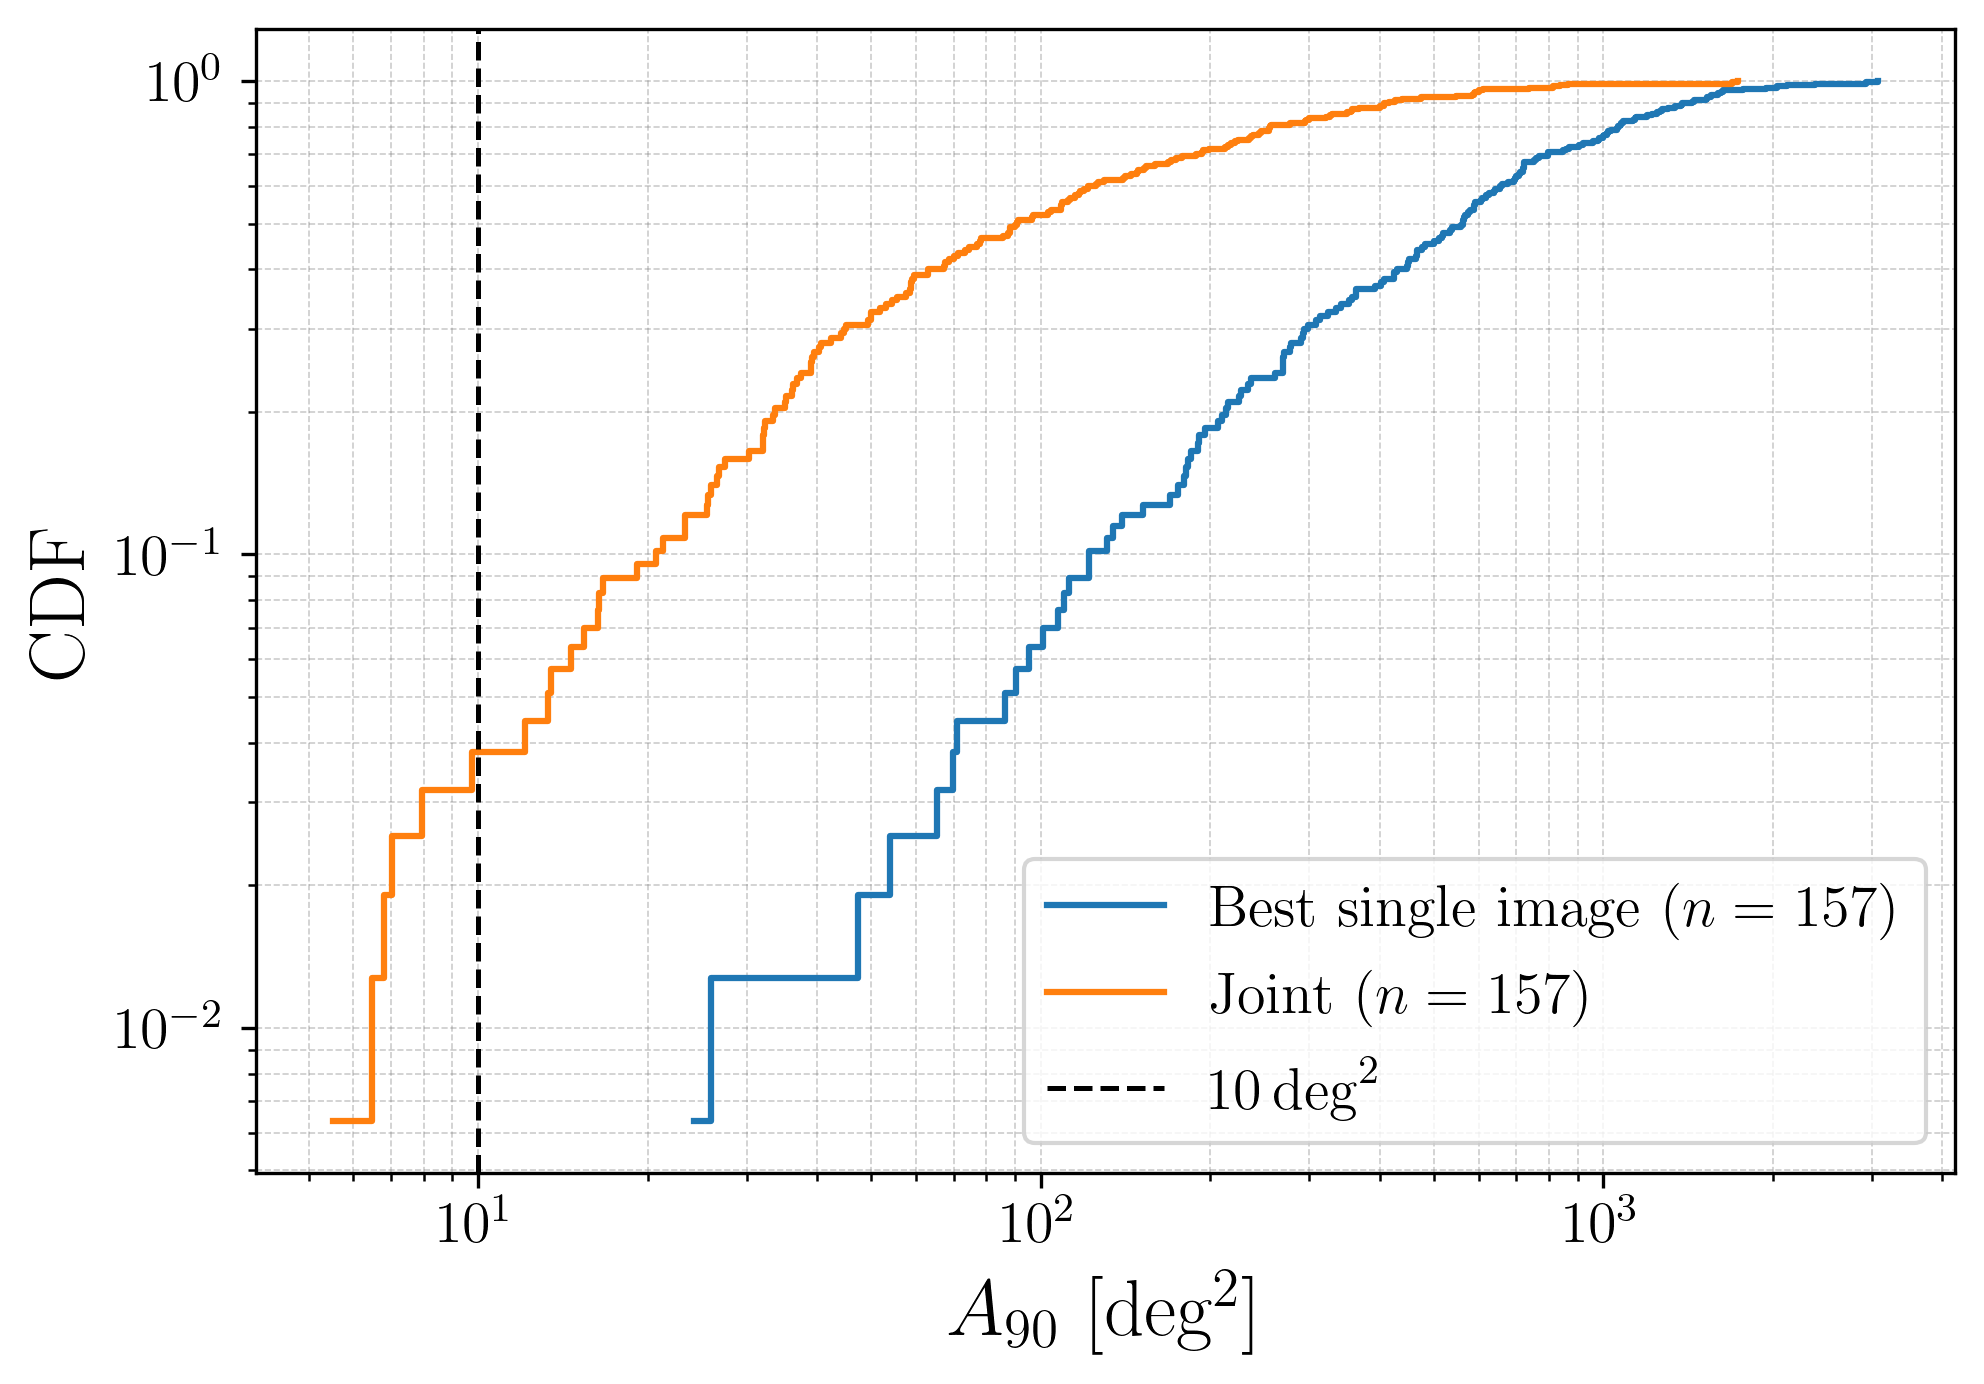
\includegraphics[width=\hsize]{Figures/cdf_90_area.png}
    \caption[CDF and PDF of $A_{90}$]{Cumulative (left) and probability
    density (right) distributions of the 90\% credible sky area, for the
    best single-image analysis and the joint analysis, across the 157
    analyzed events. The vertical dashed line marks $10\,\mathrm{deg}^2$.}
    \label{fig:cdf_pdf_area90}
\end{figure}

\subsection{Dependence on network SNR}
\label{sec:results_snr}

Figure~\ref{fig:area_vs_snr} shows $A_{90}$ as a function of the per-image
network SNR, for each image and for the joint analysis. The single-image
areas show substantial scatter at fixed SNR, reflecting the dominant role of
sky position and antenna pattern orientation, rather than SNR alone, in
setting the localization precision of a two-detector network
(\S\ref{sec:antenna_pattern}). The joint analysis consistently reduces
$A_{90}$ relative to either single image, with the largest gains occurring
for events whose single-image areas are largest to begin with.

\begin{figure}[htbp]
    \centering
    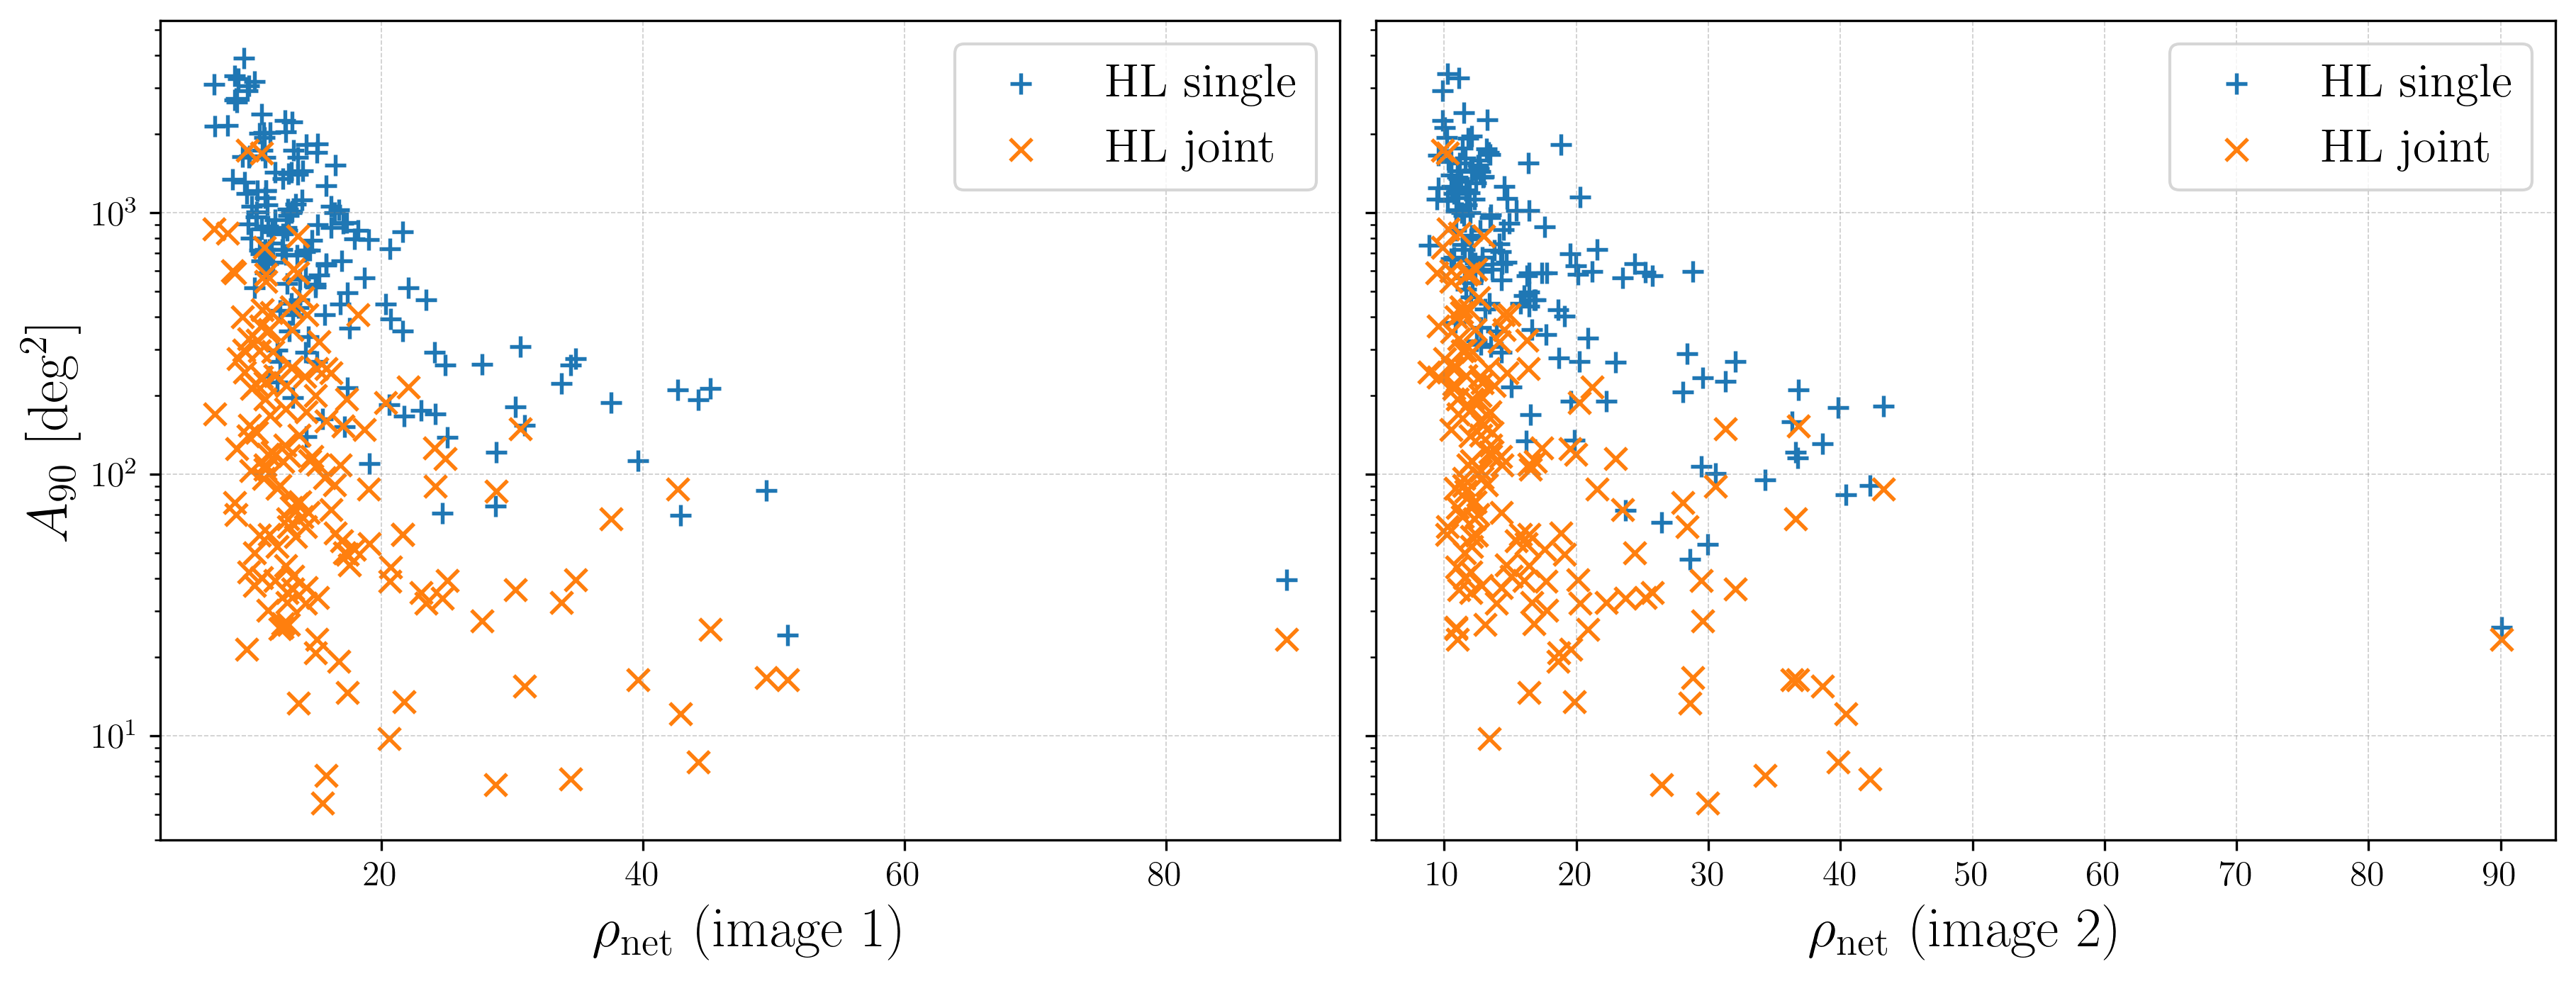
\includegraphics[width=\hsize]{Figures/sky_area_vs_snr_hl.png}
    \caption{90\% credible sky area versus network SNR for image~1 (left)
    and image~2 (right). Blue crosses: single-image analysis; orange
    crosses: joint analysis for the same event.}
    \label{fig:area_vs_snr}
\end{figure}

\subsection{Constellation localization}
\label{sec:results_constellation}

We further characterize the localization using the fraction of posterior
probability contained in the dominant IAU constellation
\citep{singer2016constellations}. For single-image analyses the median
fraction in the top constellation is $41.75\,\%$ (best of the two images).
The joint analysis raises the median to $69.3\,\%$, with $121/157$ events
($77.1\,\%$) above $50\,\%$ and $49/157$ events ($31.2\,\%$) above $90\,\%$.

Comparing against the published sky maps of 104 GWTC-5 events
\citep{ligo2026gwtc5}, we find that the joint lensed-pair analysis with only
two detectors reaches constellation fractions comparable to those achieved
by the three-detector HLV network on real data, whereas real HL-only events
are confined below $\sim 50\,\%$ (Fig.~\ref{fig:constellation_gwtc5}). This
places the improvement from the joint lensed analysis on a comparable
footing to the localization gain from adding a third detector, using only
two detectors and a repeated observation of the same source, a connection
we examine directly in \S\ref{sec:virgo}.

\begin{figure}[htbp]
    \centering
    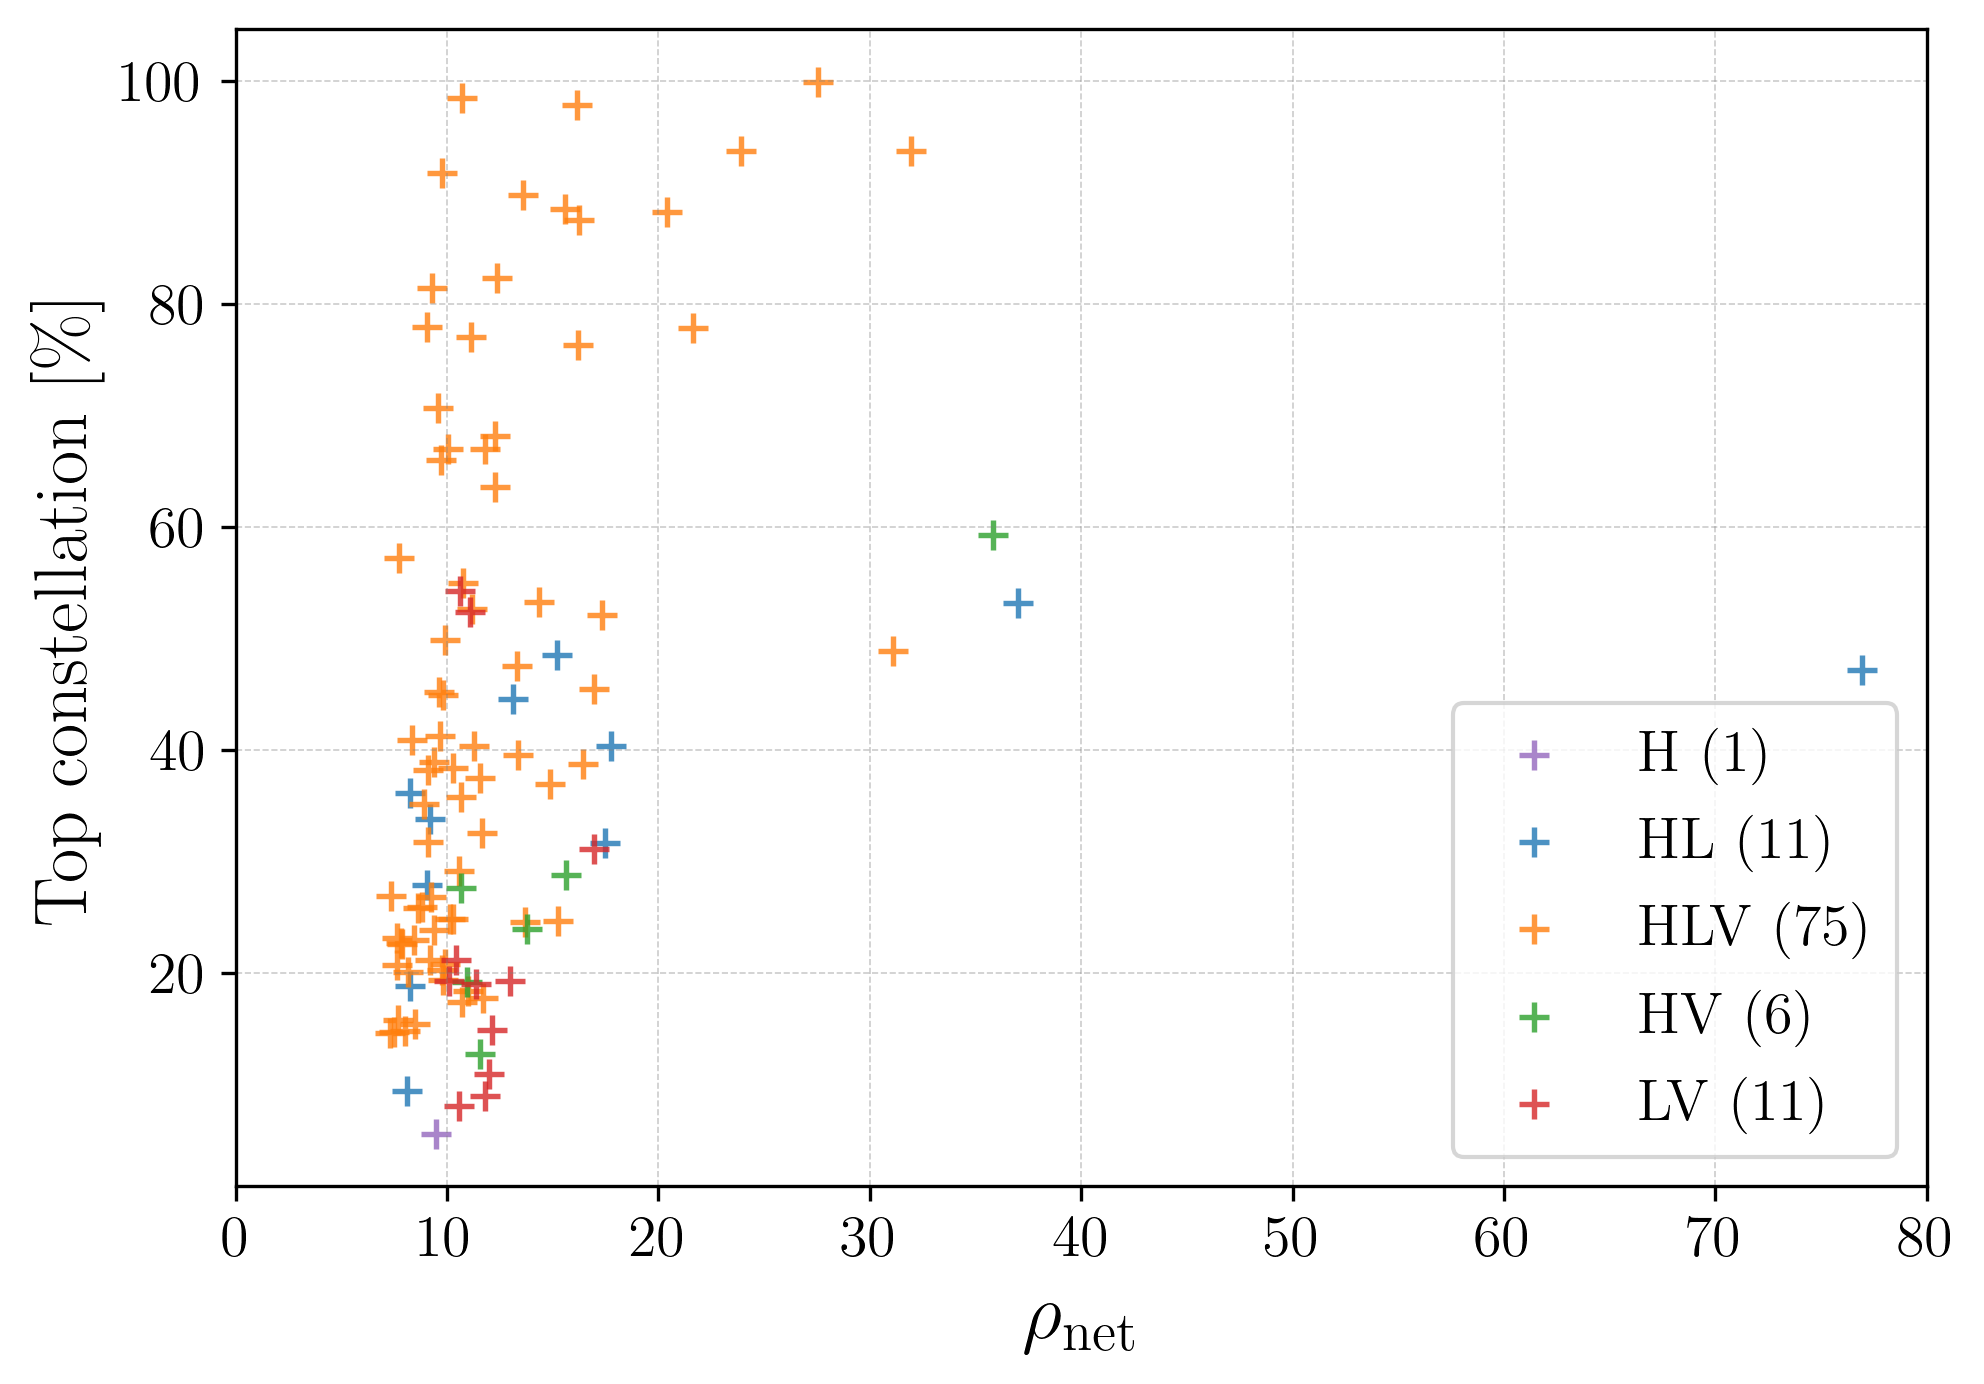
\includegraphics[width=\hsize]{Figures/constellation_vs_SNR_GWTC5.png}
    \caption{Probability fraction in the dominant constellation versus
    network SNR for 104 GWTC-5 events, colored by detector network. The HL
    subset, matching the detector configuration used in this work, is
    confined below $\sim 50\,\%$.}
    \label{fig:constellation_gwtc5}
\end{figure}

\subsection{Comparison with previous work}
\label{sec:results_comparison}

\citet{hannuksela2020localizing} demonstrated that quadruply lensed events
observed by the full LIGO/Virgo/KAGRA network can, combined with
electromagnetic constraints on the lens galaxy, be localized to one or a few
candidate host galaxies. \citet{li2026repeated} performed the first
systematic study of repeated-signal localization using
\textsc{Bayestar} sky maps on a simulated population observed with the
three-detector HLV network, finding roughly an order-of-magnitude reduction
in the 90\% credible area from combining two images. The smaller median
improvement factor found here ($5.19$) is consistent with the more
conservative two-detector configuration adopted in this work: with only H1
and L1, single-image localization already relies more heavily on antenna
pattern information than on triangulation, leaving comparatively less room
for a second image, which acts through the same antenna-pattern channel, to
improve upon it. Both studies nonetheless converge on the same qualitative
conclusion, namely that combining two lensed images yields a substantial and
consistent sky localization gain regardless of detector network or analysis
method. \S\ref{sec:virgo} tests this conclusion directly by asking how the
gain from the lensed pair interacts with growing the detector network
itself.

\section{Adding a third detector: Virgo}
\label{sec:virgo}

The results of \S\ref{sec:results_hl} isolate the gain from a coherent joint
analysis of two lensed images within a fixed two-detector network. We now
ask a complementary question: how much further does sky localization
improve when a third detector, Virgo, is added to the network, and does
that gain depend on the geometry of the event relative to the H1-L1
baseline?

\subsection{A stratified subsample, not a random one}
\label{sec:virgo_subsample}

Re-running the full 157-event population with Virgo added is
computationally prohibitive within the scope of this work. We instead
select a stratified subsample of 35 events, designed to probe four distinct
regimes of expected Virgo benefit, rather than drawing a random subset:
\texttt{core} (the 15 events with the largest fractional SNR gain from
adding V1, computed with the exact inner-product SNR estimator of
\textsc{gwsnr}), \texttt{geom} (the 10 events for which neither lensed image
is well aligned with the H1-L1 baseline, quantified by the angle between the
source direction and the baseline at each image's arrival time, so that
triangulation with H1+L1 alone is least reliable), \texttt{control} (5
events with low expected SNR gain and good H1-L1 alignment, included as a
null case), and \texttt{threshold} (5 events whose H1+L1 joint area sits
close to the $10\,\mathrm{deg}^2$ benchmark of \S\ref{sec:results_area90},
where a modest absolute change in area has an outsized practical effect on
follow-up feasibility).

Because this selection deliberately overrepresents events favorable to
Virgo, the median statistics reported below describe this stratified
subsample and \emph{must not} be compared directly to the population-level
medians of \S\ref{sec:results_hl}. Instead, every comparison in this
section is made event by event: the same 35 events are re-analyzed with the
H1+L1+V1 (HLV) network, using the Virgo O5 low-sensitivity design curve
\citep{virgo_o5_psd}, under the same pipeline, priors, and waveform model as
the H1+L1 (HL) analysis, and the two outcomes for each event are compared
directly. The full per-event table is given in
Appendix~\ref{app:virgo_table}.

\subsection{Sky area: HL versus HLV}
\label{sec:virgo_area}

Figure~\ref{fig:hl_vs_hlv_scatter} shows the joint 90\% credible area with
HLV against the same quantity with HL, for all 35 events. Every event falls
below the diagonal: adding Virgo improves the localization of every event
in the subsample, with no exceptions. The per-event improvement factor,
$\mathrm{IF}_{\rm Virgo} \equiv A_{90}^{\rm joint,\,HL}/A_{90}^{\rm joint,\,HLV}$,
has a median of $13.3$ across the subsample (range $2.4$--$93.8$), and the
median joint area drops from $71.2\,\mathrm{deg}^2$ (HL) to
$8.8\,\mathrm{deg}^2$ (HLV). Twenty of the 35 events ($57.1\,\%$) fall below
the $10\,\mathrm{deg}^2$ benchmark with Virgo, compared to a single event
with H1+L1 alone. The median dominant-constellation fraction rises
correspondingly, from $73.3\,\%$ (HL) to $99.5\,\%$ (HLV).

\begin{figure}[htbp]
    \centering
    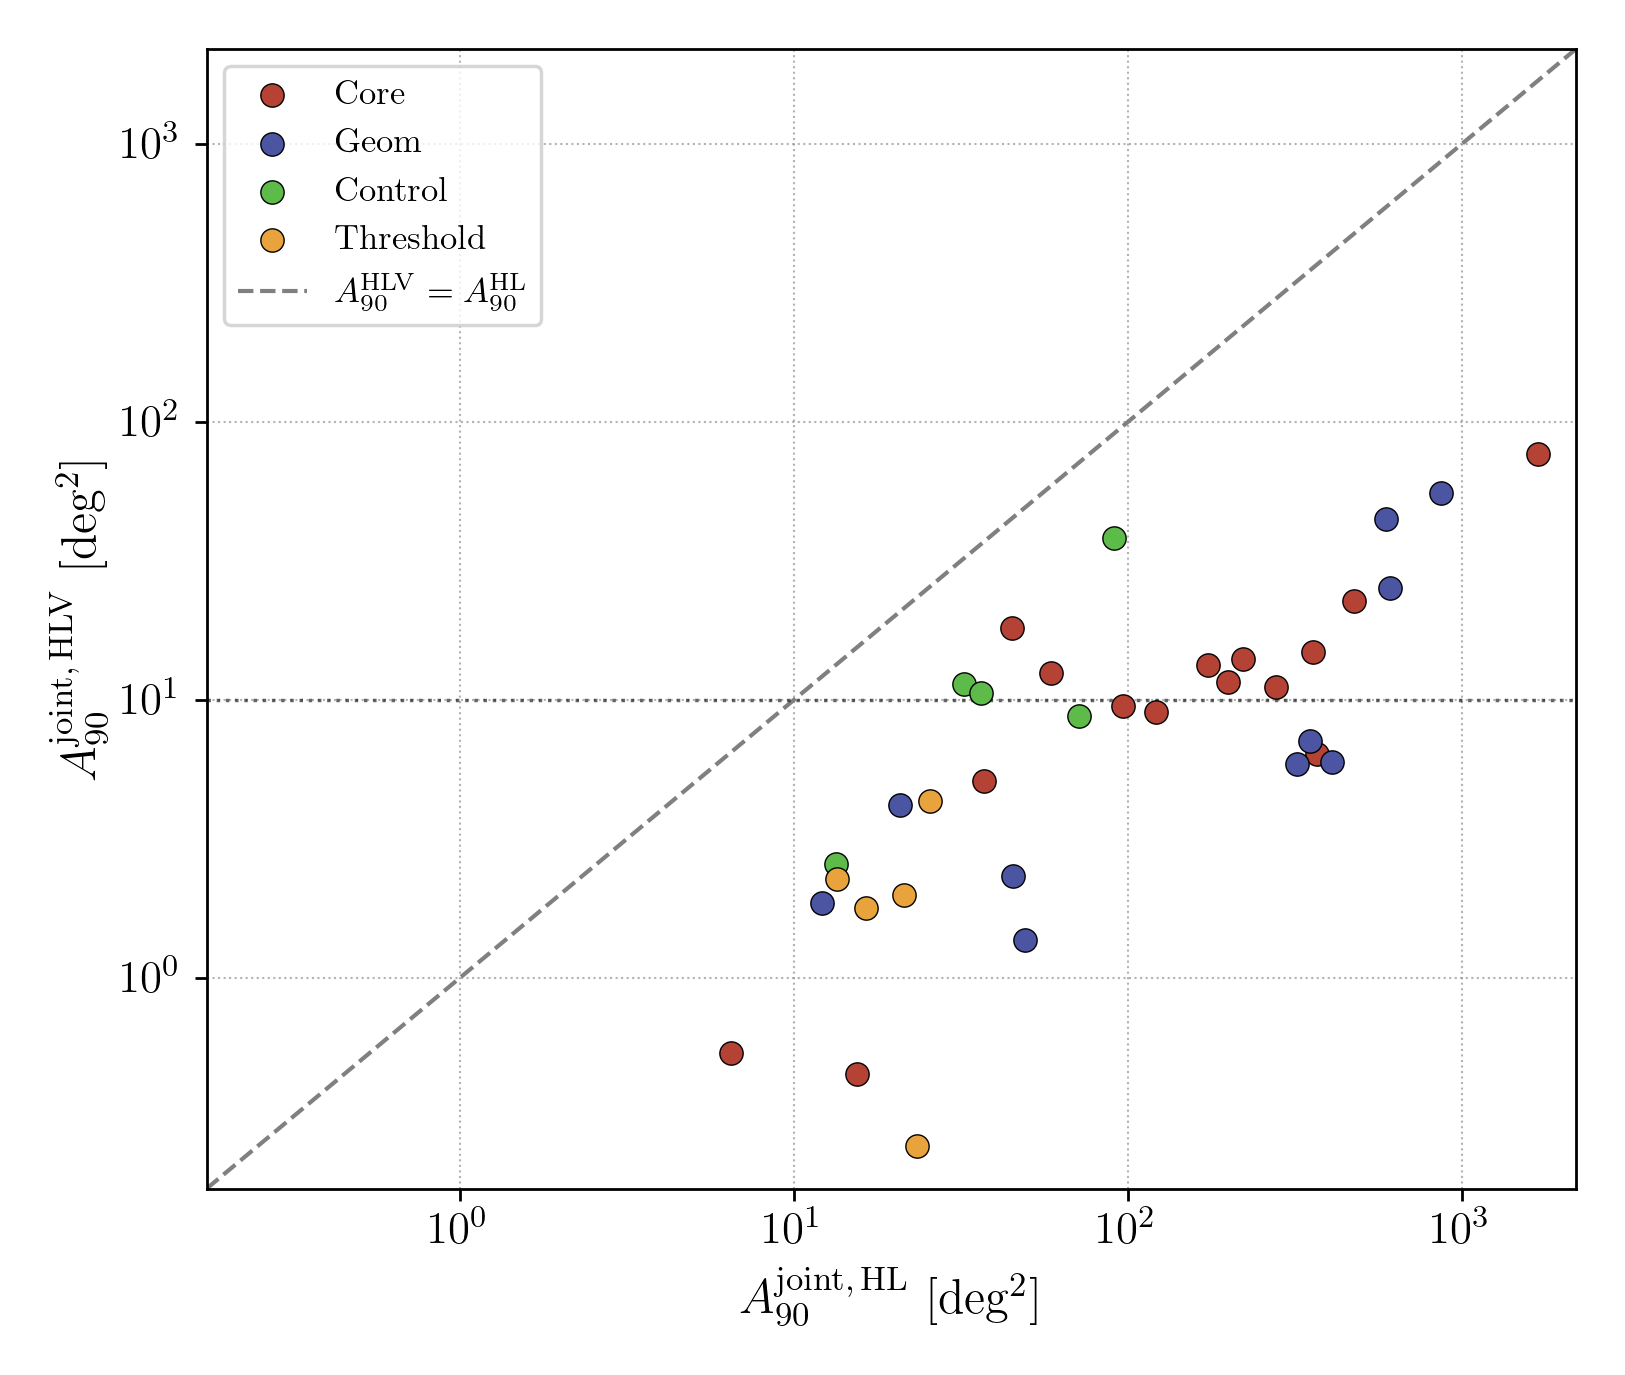
\includegraphics[width=\hsize]{Figures/hl_vs_hlv_area90_scatter.png}
    \caption{Joint 90\% credible area with H1+L1+V1 (HLV) versus H1+L1
    (HL), for the 35-event stratified subsample, colored by selection
    group. The dashed line marks equal area; every point falls below it.
    The dotted line marks $10\,\mathrm{deg}^2$.}
    \label{fig:hl_vs_hlv_scatter}
\end{figure}

Figure~\ref{fig:hl_vs_hlv_slopechart} shows the same comparison per event,
as a slope chart grouped by selection category, making the heterogeneity of
the gain across groups directly visible: the \texttt{core} and
\texttt{geom} groups, selected respectively for high expected SNR gain and
for poor H1-L1 geometric alignment, show the largest improvements (median
$\mathrm{IF}_{\rm Virgo} = 15.8$ and $21.9$), while the \texttt{control}
group, selected as a null case of low SNR gain and favorable H1-L1
alignment, shows the smallest (median $3.4$). The \texttt{threshold} group,
selected independently of either criterion, falls in between (median
$9.2$). This ordering confirms that the selection criteria used to build the
subsample track the physical drivers of the Virgo gain: events that are
geometrically degenerate under H1+L1, or that happen to be loud in Virgo,
benefit the most, while events already well constrained by H1+L1
triangulation gain comparatively little from a third detector.

\begin{figure}[htbp]
    \centering
    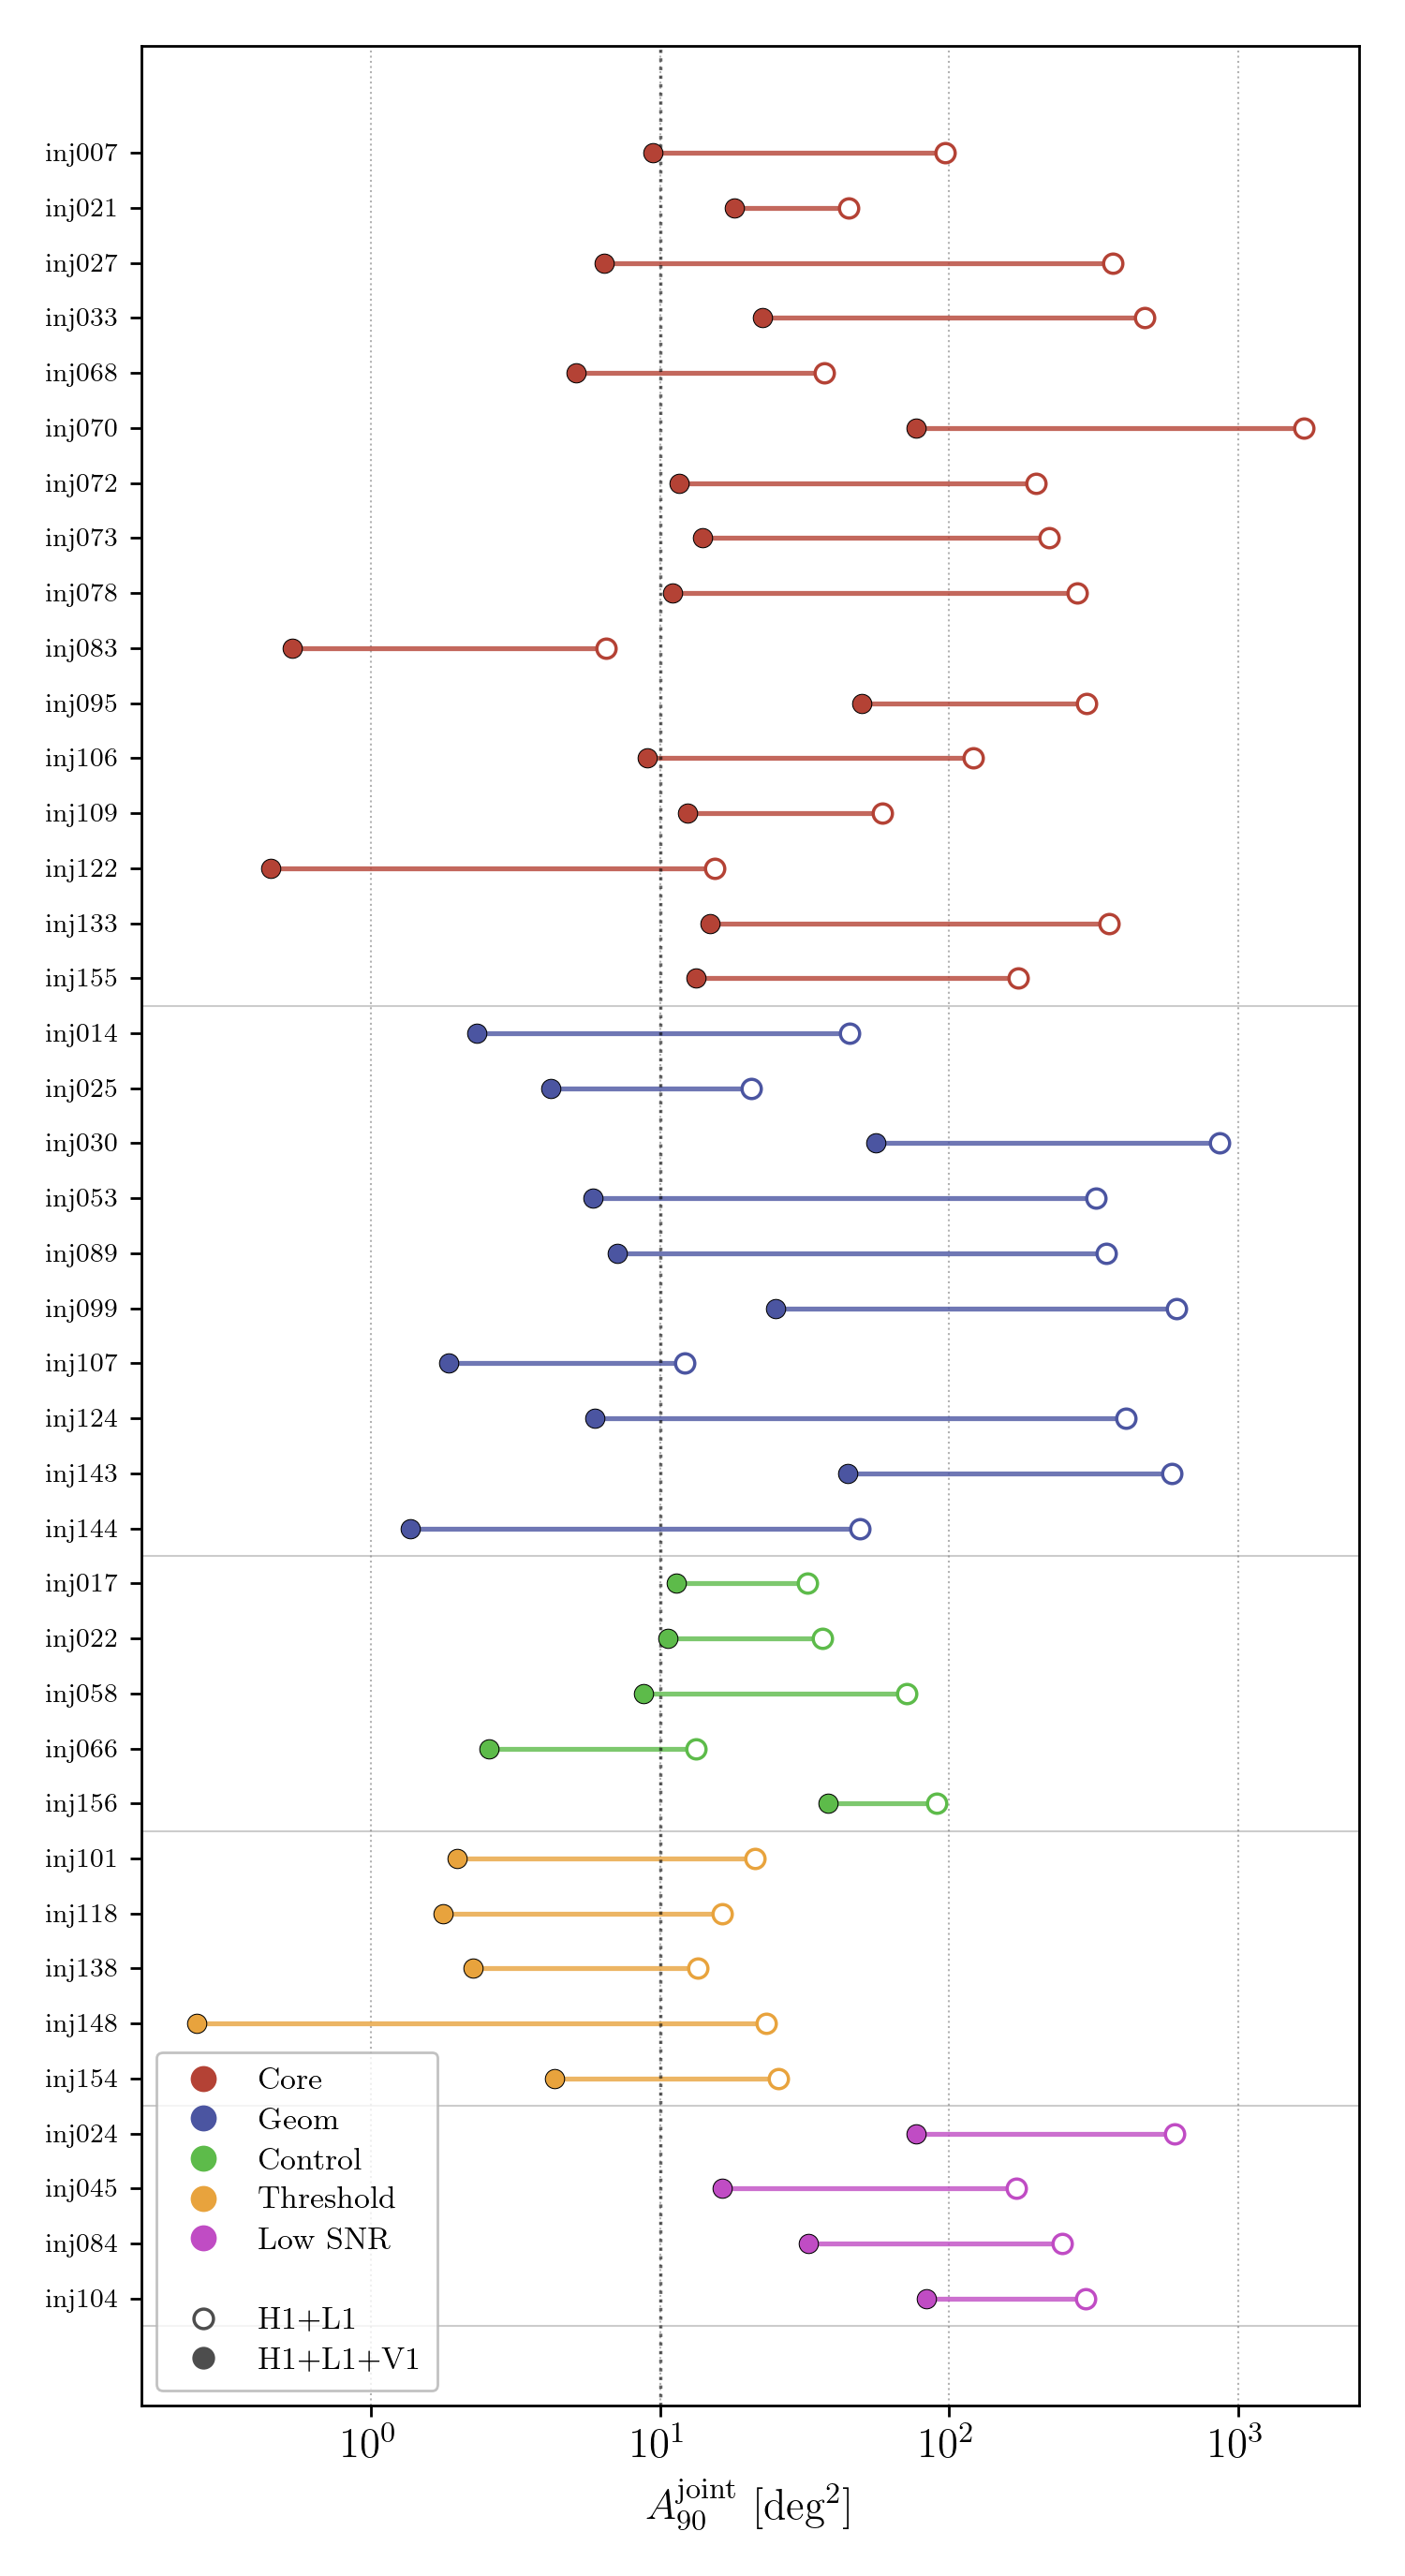
\includegraphics[width=\hsize]{Figures/hl_vs_hlv_area90_slopechart.png}
    \caption{Joint 90\% credible area for each of the 35 events, with H1+L1
    (open markers) and H1+L1+V1 (filled markers), grouped by selection
    category. The dotted line marks $10\,\mathrm{deg}^2$.}
    \label{fig:hl_vs_hlv_slopechart}
\end{figure}

\subsection{The diminishing, but still positive, value of the lensed pair}
\label{sec:virgo_diminishing}

A natural question is whether the gain from combining two lensed images,
the central result of \S\ref{sec:results_hl}, persists once a third
detector is already available. Within the HL network, the median value of
$\mathrm{IF}_{\rm joint}$ (Eq.~\eqref{eq:if_joint}) for this 35-event
subsample is $4.68$, consistent with the $5.19$ found for the full
157-event population (\S\ref{sec:results_area90}) and confirming that the
subsample is not biased with respect to this particular metric. Within the
HLV network, the same quantity, which we denote $\mathrm{IF}_{\rm joint}^{\rm HLV}$
to distinguish it from its HL counterpart $\mathrm{IF}_{\rm joint}^{\rm HL}$,
drops to $2.20$.

This does not mean that combining the two lensed images becomes
uninformative once Virgo is added. Every event in the subsample still
benefits from the joint analysis within the HLV network itself
(Appendix~\ref{app:virgo_table}), and the absolute localization achieved by
the HLV joint analysis remains, by a wide margin, the best result available
for any of these events. What the drop in $\mathrm{IF}_{\rm joint}$
indicates is that the specific role played by the second lensed image,
namely supplying an independent triangulation baseline through its
different arrival time and antenna-pattern orientation, is partially
subsumed once a third detector already provides that information directly.
The lensed-pair technique and a richer detector network are therefore
complementary rather than redundant: the former matters most precisely in
the regime probed by the \texttt{geom} group, where the detector network
alone is geometrically degenerate, and its marginal contribution shrinks,
without vanishing, as the network's own triangulation power increases.

\subsection{Comparison with the literature}
\label{sec:virgo_comparison}

These results extend the central finding of \S\ref{sec:results_comparison}
along a second, complementary axis: while \S\ref{sec:results_hl} shows that
repeating an observation through a lensed image pair substantially improves
localization within a fixed detector network, the present section shows
that growing the detector network itself delivers a comparable, and in the
most favorable cases much larger, improvement, and that the two strategies
interact in the physically expected way, each compensating most for the
specific geometric limitations the other leaves unaddressed.




%%%%%%%%%%%%%%%%%%%%%%%%%%%%%%%%%%%%%%%%%%%%%%%%%%%%%%%%%%%%%%
\section{Conclusions}
Lorem ipsum dolor sit amet,
consectetuer adipiscing elit. In hac habitasse platea dictumst. In-
teger tempus convallis augue. Etiam facilisis.

%%%%%%%%%%%%%%%%%%%%%%%%%%%%%%%%%%%%%%%%%%%%%%%%%%%%%%%%%%%%%%
\begin{acknowledgements}
      Part of this work was supported by \emph{ESO}, project
      number Ts~17/2--1.
\end{acknowledgements}




%%%%%%%%%%%%%%%%%%%%%%%%%%%%%%%%%%%%%%%%%%%%%%%%%%%%%%%%%%%%%%
% WARNING
% Please note that we have included the references below in
% order to compile the document, but we ask you to:
%
% - use BibTeX with the regular commands:
%   \bibliographystyle{aa} % style aa.bst
%   \bibliography{Yourfile} % your references Yourfile.bib
% - join the .bib files when you upload your source files
%%%%%%%%%%%%%%%%%%%%%%%%%%%%%%%%%%%%%%%%%%%%%%%%%%%%%%%%%%%%%%

\begin{thebibliography}{}

  \bibitem[Baker(1966)]{baker} Baker, N. 1966,
      in Stellar Evolution,
      ed.\ R. F. Stein,\& A. G. W. Cameron
      (Plenum, New York) 333

   \bibitem[Balluch(1988)]{balluch} Balluch, M. 1988,
      A\&A, 200, 58

   \bibitem[Cox(1980)]{cox} Cox, J. P. 1980,
      Theory of Stellar Pulsation
      (Princeton University Press, Princeton) 165

   \bibitem[Cox(1969)]{cox69} Cox, A. N.,\& Stewart, J. N. 1969,
      Academia Nauk, Scientific Information 15, 1

   \bibitem[Mizuno(1980)]{mizuno} Mizuno H. 1980,
      Prog. Theor. Phys., 64, 544
   
   \bibitem[Tscharnuter(1987)]{tscharnuter} Tscharnuter W. M. 1987,
      A\&A, 188, 55
  
   \bibitem[Terlevich(1992)]{terlevich} Terlevich, R. 1992, in ASP Conf. Ser. 31,
      Relationships between Active Galactic Nuclei and Starburst Galaxies,
      ed. A. V. Filippenko, 13

   \bibitem[Yorke(1980a)]{yorke80a} Yorke, H. W. 1980a,
      A\&A, 86, 286

   \bibitem[Zheng(1997)]{zheng} Zheng, W., Davidsen, A. F., Tytler, D. \& Kriss, G. A.
      1997, preprint
\end{thebibliography}


% %%%%%%%%%%%%%%%%%%%%%%%%%%%%%%%%%%%%%%%%%%%%%%%%%%%%%%%%%%%%%%
% Example below of non-structurated natbib references  
% To use the v8.3 macros with this form of composition of bibliography,
% the option "bibyear" should be added to the command line
% "\documentclass[bibyear]{aa}".
% %%%%%%%%%%%%%%%%%%%%%%%%%%%%%%%%%%%%%%%%%%%%%%%%%%%%%%%%%%%%%%

% \begin{thebibliography}{}

%   \bibitem[1966]{baker} Baker, N. 1966,
%       in Stellar Evolution,
%       ed.\ R. F. Stein,\& A. G. W. Cameron
%       (Plenum, New York) 333

%    \bibitem[1988]{balluch} Balluch, M. 1988,
%       A\&A, 200, 58

%    \bibitem[1980]{cox} Cox, J. P. 1980,
%       Theory of Stellar Pulsation
%       (Princeton University Press, Princeton) 165

%    \bibitem[1969]{cox69} Cox, A. N.,\& Stewart, J. N. 1969,
%       Academia Nauk, Scientific Information 15, 1

%    \bibitem[1980]{mizuno} Mizuno H. 1980,
%       Prog. Theor. Phys., 64, 544
   
%    \bibitem[1987]{tscharnuter} Tscharnuter W. M. 1987,
%       A\&A, 188, 55
  
%    \bibitem[1992]{terlevich} Terlevich, R. 1992, in ASP Conf. Ser. 31,
%       Relationships between Active Galactic Nuclei and Starburst Galaxies,
%       ed. A. V. Filippenko, 13

%    \bibitem[1980a]{yorke80a} Yorke, H. W. 1980a,
%       A\&A, 86, 286

%    \bibitem[1997]{zheng} Zheng, W., Davidsen, A. F., Tytler, D. \& Kriss, G. A.
%       1997, preprint
% \end{thebibliography}




%%%%%%%%%%%%%%%%%%%%%%%%%%%%%%%%%%%%%%%%%%%%%%%%%%%%%%%%%%%%%%%
% Appendices must be placed after   \end{thebibliography}
% They will be placed automatically on a new page.
%%%%%%%%%%%%%%%%%%%%%%%%%%%%%%%%%%%%%%%%%%%%%%%%%%%%%%%%%%%%%%%
\begin{appendix}
%%%%%%%%%%%%%%%%%%%%%%%%%%%%%%%%%%%%%%%%%%%%%%%%%%%%%%%%%%%%%%%
% In the PDF output, floats should be placed
% under their own appendix, not before the title, nor after the
% title of the next appendix.

% In short appendices, onecolumn floats (\figure*
% or \table*) will generate a blank page.
% To prevent this behaviour, a few examples are provided here. 

% In case you have a lot of floating objects for little text and the 
% LaTeX engine moves the floats away from their context, the command
% \FloatBarrier of the “placeins” package will empty the
% float buffer and place all stored floats in the continuity.

% If you still encounter problems with wide floats placement,
% just use the onecolumn environment throughout the appendices.
%%%%%%%%%%%%%%%%%%%%%%%%%%%%%%%%%%%%%%%%%%%%%%%%%%%%%%%%%%%%%%%




\onecolumn
\section{Full per-event results for the Virgo subsample}
\label{app:virgo_table}

Table~\ref{tab:virgo_35events} lists, for each of the 35 events analyzed
with H1+L1+V1 (\S\ref{sec:virgo}), the selection group, the joint 90\%
credible area with H1+L1 (HL) and H1+L1+V1 (HLV), the per-event improvement
factor from adding Virgo to the joint analysis ($\mathrm{IF}_{\rm Virgo}$),
and the improvement factor from combining the two lensed images within each
network separately ($\mathrm{IF}_{\rm joint}^{\rm HL}$,
$\mathrm{IF}_{\rm joint}^{\rm HLV}$), as discussed in
\S\ref{sec:virgo_diminishing}.



\begin{table}[ht!]
\centering
\caption{Per-event sky-area results for the 35-event Virgo subsample.}
\label{tab:virgo_35events}
\begin{tabular}{llrrrrr}
\hline\hline
Event & Group & $A_{90}^{\rm joint,\,HL}$ & $A_{90}^{\rm joint,\,HLV}$ &
$\mathrm{IF}_{\rm Virgo}$ & $\mathrm{IF}_{\rm joint}^{\rm HL}$ &
$\mathrm{IF}_{\rm joint}^{\rm HLV}$ \\
 & & [deg$^2$] & [deg$^2$] & & & \\
\hline
inj027 & Core & 367.8 & 6.4 & 57.64 & 1.89 & 2.20 \\
inj122 & Core & 15.4 & 0.4 & 34.36 & 8.48 & 0.68 \\
inj078 & Core & 276.9 & 11.1 & 25.02 & 7.66 & 2.69 \\
inj133 & Core & 357.3 & 14.8 & 24.07 & 1.70 & 2.26 \\
inj070 & Core & 1690.2 & 76.7 & 22.03 & 1.41 & 2.15 \\
inj033 & Core & 473.0 & 22.5 & 20.98 & 3.06 & 1.78 \\
inj072 & Core & 199.4 & 11.6 & 17.19 & 2.68 & 2.37 \\
inj073 & Core & 221.3 & 14.0 & 15.76 & 3.06 & 1.70 \\
inj106 & Core & 121.4 & 9.0 & 13.48 & 6.98 & 1.31 \\
inj155 & Core & 173.7 & 13.3 & 13.03 & 5.51 & 1.29 \\
inj083 & Core & 6.5 & 0.5 & 12.14 & 10.09 & 2.14 \\
inj007 & Core & 96.6 & 9.4 & 10.22 & 10.12 & 1.47 \\
inj068 & Core & 36.9 & 5.1 & 7.23 & 3.78 & 2.67 \\
inj109 & Core & 58.8 & 12.4 & 4.72 & 4.03 & 2.29 \\
inj021 & Core & 44.7 & 18.1 & 2.47 & 11.15 & 1.58 \\
\noalign{\smallskip}
inj124 & Geom & 407.9 & 5.9 & 68.61 & 1.77 & 2.74 \\
inj053 & Geom & 321.2 & 5.9 & 54.76 & 1.80 & 1.58 \\
inj089 & Geom & 350.5 & 7.1 & 49.23 & 3.07 & 2.43 \\
inj144 & Geom & 49.2 & 1.4 & 36.21 & 8.18 & 2.45 \\
inj099 & Geom & 609.7 & 25.1 & 24.28 & 2.14 & 2.93 \\
inj014 & Geom & 45.1 & 2.3 & 19.42 & 8.05 & 1.83 \\
inj030 & Geom & 865.1 & 55.5 & 15.58 & 1.85 & 1.59 \\
inj143 & Geom & 590.9 & 44.5 & 13.27 & 2.02 & 1.38 \\
inj107 & Geom & 12.1 & 1.9 & 6.53 & 5.76 & 1.81 \\
inj025 & Geom & 20.7 & 4.2 & 4.96 & 13.42 & 2.35 \\
\noalign{\smallskip}
inj058 & Control & 71.2 & 8.8 & 8.13 & 4.71 & 6.05 \\
inj066 & Control & 13.3 & 2.6 & 5.22 & 3.55 & 6.47 \\
inj022 & Control & 36.3 & 10.6 & 3.42 & 7.42 & 3.93 \\
inj017 & Control & 32.3 & 11.4 & 2.84 & 5.91 & 2.26 \\
inj156 & Control & 90.7 & 38.2 & 2.38 & 4.68 & 2.93 \\
\noalign{\smallskip}
inj148 & Threshold & 23.3 & 0.2 & 93.77 & 1.11 & 1.65 \\
inj101 & Threshold & 21.3 & 2.0 & 10.79 & 8.92 & 1.29 \\
inj118 & Threshold & 16.4 & 1.8 & 9.24 & 1.48 & 2.75 \\
inj138 & Threshold & 13.5 & 2.3 & 5.96 & 10.00 & 1.93 \\
inj154 & Threshold & 25.6 & 4.3 & 5.95 & 10.58 & 4.01 \\
\hline
\end{tabular}
\end{table}


\FloatBarrier %\usepackage{placeins}
\twocolumn













%____________________________________________________________
%       Wide floats at the start of an appendix: first method
%-------------------------------------------------------------
% To prevent a blank page after the start of an appendix:
% - Switch to one \onecolumn first
% - Declare the section title
% - Declare the onecolumn float with the parameter [ht!]
% - Revert to \twocolumn at the end of the section

\onecolumn
\section{Wide tables and figures after an appendix title: recommended method}
%

In the PDF output, \underline{floats should be placed
under their own appendix}, not before the title, nor after the
title of the next appendix. In short appendices, one-column floats
\{figure*\} or \{table*\} will generate
a blank page. To prevent this behaviour, we recommend to switch
to \textbackslash onecolumn and set the [ht!] parameter 
in your floats: please check the \LaTeX code of this appendix.\\

In case you have a lot of floating objects for little text and the 
\LaTeX engine moves the floats away from their context, the command
\textbackslash FloatBarrier of the “placeins” package will empty the
float buffer and place all stored floats in the continuity. If you still encounter problems with wide floats placement, just use the \textbackslash onecolumn
environment throughout the appendices.


\begin{figure*}[ht!]
    \centering
     \resizebox{12cm}{12cm}
    {
\includegraphics {figure.eps}}
     \caption{A one-column \{figure*\}[ht!] after a section title.
      If text follows like below, it is easier to finish the section in
      \textbackslash onecolumn. If needed, you may revert to \textbackslash
      twocolumn when reaching the next page.}
      \label{fig5ap}
\end{figure*}


% If text follows like so 
\lipsum[1-2]
% it is easier to finish the page in onecolumn and revert to
% twocolumn when starting the next page if needed.}


\FloatBarrier %\usepackage{placeins}
\twocolumn
%____________________________________________________________
%       Wide floats at the start of an appendix: second method
%-------------------------------------------------------------
% To prevent a blank page, a second method is:
% - Declare the onecolumn float *
% - Declare the section under the float
% However, this method should be reserved to appendices
% containing only onecolumn tables or figures.
\begin{table*}[ht!]
\section{Wide tables and figures after an appendix title: alternate method}
%

To prevent a blank page, a second method is to insert
the appendix title \underline{after} declaring the onecolumn float.
\newline This method should be reserved to appendices
containing only one-column floats\{figure*\} or \{table*\}
and no text.

\caption {A one-column \{table*\} \newline}
\label{table:2} 
\centering
\begin{tabular}{crrlcl}
\hline\hline             
ISO-L1551 & $F_{6.7}$~[mJy] & $\alpha_{6.7-14.3}$
& YSO type$^{d}$ & Status & Comments\\
\hline
  \multicolumn{6}{c}{\it New YSO candidates}\\ % To combine 6 columns into a single one
\hline
  1 & 1.56 $\pm$ 0.47 & --    & Class II$^{c}$ & New & Mid\\
  2 & 0.79:           & 0.97: & Class II ?     & New & \\
  3 & 4.95 $\pm$ 0.68 & 3.18  & Class II / III & New & \\
  5 & 1.44 $\pm$ 0.33 & 1.88  & Class II       & New & \\
  1 & 1.56 $\pm$ 0.47 & --    & Class II$^{c}$ & New & Mid\\
  2 & 0.79:           & 0.97: & Class II ?     & New & \\
  3 & 4.95 $\pm$ 0.68 & 3.18  & Class II / III & New & \\
  5 & 1.44 $\pm$ 0.33 & 1.88  & Class II       & New & \\
  1 & 1.56 $\pm$ 0.47 & --    & Class II$^{c}$ & New & Mid\\
  2 & 0.79:           & 0.97: & Class II ?     & New & \\
  3 & 4.95 $\pm$ 0.68 & 3.18  & Class II / III & New & \\
  5 & 1.44 $\pm$ 0.33 & 1.88  & Class II       & New & \\
  1 & 1.56 $\pm$ 0.47 & --    & Class II$^{c}$ & New & Mid\\
  2 & 0.79:           & 0.97: & Class II ?     & New & \\
  3 & 4.95 $\pm$ 0.68 & 3.18  & Class II / III & New & \\
  5 & 1.44 $\pm$ 0.33 & 1.88  & Class II       & New & \\

  2 & 0.79:           & 0.97: & Class II ?     & New & \\
  3 & 4.95 $\pm$ 0.68 & 3.18  & Class II / III & New & \\
  5 & 1.44 $\pm$ 0.33 & 1.88  & Class II       & New & \\
  1 & 1.56 $\pm$ 0.47 & --    & Class II$^{c}$ & New & Mid\\
  2 & 0.79:           & 0.97: & Class II ?     & New & \\
  3 & 4.95 $\pm$ 0.68 & 3.18  & Class II / III & New & \\
  5 & 1.44 $\pm$ 0.33 & 1.88  & Class II       & New & \\
  1 & 1.56 $\pm$ 0.47 & --    & Class II$^{c}$ & New & Mid\\
  2 & 0.79:           & 0.97: & Class II ?     & New & \\
  3 & 4.95 $\pm$ 0.68 & 3.18  & Class II / III & New & \\
  5 & 1.44 $\pm$ 0.33 & 1.88  & Class II       & New & \\
  1 & 1.56 $\pm$ 0.47 & --    & Class II$^{c}$ & New & Mid\\
  2 & 0.79:           & 0.97: & Class II ?     & New & \\
  3 & 4.95 $\pm$ 0.68 & 3.18  & Class II / III & New & \\
  5 & 1.44 $\pm$ 0.33 & 1.88  & Class II       & New & \\
\hline
  \multicolumn{6}{c}{\it Previously known YSOs} \\
\hline
  61 & 0.89 $\pm$ 0.58 & 1.77 & Class I & \object{HH 30} & Circumstellar disk\\
  96 & 38.34 $\pm$ 0.71 & 37.5& Class II& MHO 5          & Spectral type\\
\hline
\end{tabular}
\end{table*}


\FloatBarrier %\usepackage{placeins}
\twocolumn
%____________________________________________________________
% A long table in appendix
%------------------------------------------------------------
% This is the start of the page
\onecolumn
\section{Long tables in appendices}
For long tables (multipage) in appendices, we use the method described in appendix A.
For long landscape tables, please refer to Appendix E.
\begin{longtable}{lllrrr}
%

\caption{A long table}\\
\label{ltapp} \\
\hline\hline
Catalogue& $M_{V}$ & Spectral & Distance & Mode & Count Rate \\
\hline
\endfirsthead
\caption{continued.}\\
\hline
Catalogue& $M_{V}$ & Spectral & Distance & Mode & Count Rate \\
\hline
\endhead
\hline
\endfoot
%%
Gl 33    & 6.37 & K2 V & 7.46 & S & 0.043170\\
Gl 66AB  & 6.26 & K2 V & 8.15 & S & 0.260478\\
Gl 68    & 5.87 & K1 V & 7.47 & P & 0.026610\\
         &      &      &      & H & 0.008686\\
Gl 86
\footnote{Source not included in the HRI catalog. See Sect.~5.4.2 for details.}
         & 5.92 & K0 V & 10.91& S & 0.058230\\
                  & 5.92 & K0 V & 10.91& S & 0.058230\\
Gl 33    & 6.37 & K2 V & 7.46 & S & 0.043170\\
Gl 66AB  & 6.26 & K2 V & 8.15 & S & 0.260478\\
Gl 68    & 5.87 & K1 V & 7.47 & P & 0.026610\\
         &      &      &      & H & 0.008686\\
Gl 86    & 5.92 & K0 V & 10.91& S & 0.058230\\            & 5.92 & K0 V & 10.91& S & 0.058230\\
Gl 33    & 6.37 & K2 V & 7.46 & S & 0.043170\\
Gl 66AB  & 6.26 & K2 V & 8.15 & S & 0.260478\\
Gl 68    & 5.87 & K1 V & 7.47 & P & 0.026610\\
         &      &      &      & H & 0.008686\\
Gl 86    & 5.92 & K0 V & 10.91& S & 0.058230\\            & 5.92 & K0 V & 10.91& S & 0.058230\\
Gl 33    & 6.37 & K2 V & 7.46 & S & 0.043170\\
Gl 66AB  & 6.26 & K2 V & 8.15 & S & 0.260478\\
Gl 68    & 5.87 & K1 V & 7.47 & P & 0.026610\\
         &      &      &      & H & 0.008686\\
Gl 86    & 5.92 & K0 V & 10.91& S & 0.058230\\            & 5.92 & K0 V & 10.91& S & 0.058230\\
Gl 33    & 6.37 & K2 V & 7.46 & S & 0.043170\\
Gl 66AB  & 6.26 & K2 V & 8.15 & S & 0.260478\\
Gl 68    & 5.87 & K1 V & 7.47 & P & 0.026610\\
         &      &      &      & H & 0.008686\\
Gl 86    & 5.92 & K0 V & 10.91& S & 0.058230\\            & 5.92 & K0 V & 10.91& S & 0.058230\\
Gl 33    & 6.37 & K2 V & 7.46 & S & 0.043170\\
Gl 66AB  & 6.26 & K2 V & 8.15 & S & 0.260478\\
Gl 68    & 5.87 & K1 V & 7.47 & P & 0.026610\\
         &      &      &      & H & 0.008686\\
Gl 86    & 5.92 & K0 V & 10.91& S & 0.058230\\            & 5.92 & K0 V & 10.91& S & 0.058230\\
Gl 33    & 6.37 & K2 V & 7.46 & S & 0.043170\\
Gl 66AB  & 6.26 & K2 V & 8.15 & S & 0.260478\\
Gl 68    & 5.87 & K1 V & 7.47 & P & 0.026610\\
         &      &      &      & H & 0.008686\\
Gl 86    & 5.92 & K0 V & 10.91& S & 0.058230\\            & 5.92 & K0 V & 10.91& S & 0.058230\\
Gl 33    & 6.37 & K2 V & 7.46 & S & 0.043170\\
Gl 66AB  & 6.26 & K2 V & 8.15 & S & 0.260478\\
Gl 68    & 5.87 & K1 V & 7.47 & P & 0.026610\\
         &      &      &      & H & 0.008686\\
Gl 86    & 5.92 & K0 V & 10.91& S & 0.058230\\            & 5.92 & K0 V & 10.91& S & 0.058230\\
Gl 33    & 6.37 & K2 V & 7.46 & S & 0.043170\\
Gl 66AB  & 6.26 & K2 V & 8.15 & S & 0.260478\\
Gl 68    & 5.87 & K1 V & 7.47 & P & 0.026610\\
         &      &      &      & H & 0.008686\\
Gl 86    & 5.92 & K0 V & 10.91& S & 0.058230\\            & 5.92 & K0 V & 10.91& S & 0.058230\\
Gl 33    & 6.37 & K2 V & 7.46 & S & 0.043170\\
Gl 66AB  & 6.26 & K2 V & 8.15 & S & 0.260478\\
Gl 68    & 5.87 & K1 V & 7.47 & P & 0.026610\\
         &      &      &      & H & 0.008686\\
Gl 86    & 5.92 & K0 V & 10.91& S & 0.058230\\
         & 5.92 & K0 V & 10.91& S & 0.058230\\
Gl 33    & 6.37 & K2 V & 7.46 & S & 0.043170\\
Gl 66AB  & 6.26 & K2 V & 8.15 & S & 0.260478\\
Gl 68    & 5.87 & K1 V & 7.47 & P & 0.026610\\
         &      &      &      & H & 0.008686\\
Gl 86    & 5.92 & K0 V & 10.91& S & 0.058230\\            & 5.92 & K0 V & 10.91& S & 0.058230\\
Gl 33    & 6.37 & K2 V & 7.46 & S & 0.043170\\
Gl 66AB  & 6.26 & K2 V & 8.15 & S & 0.260478\\
Gl 68    & 5.87 & K1 V & 7.47 & P & 0.026610\\
         &      &      &      & H & 0.008686\\
Gl 86    & 5.92 & K0 V & 10.91& S & 0.058230\\
         & 5.92 & K0 V & 10.91& S & 0.058230\\
Gl 33    & 6.37 & K2 V & 7.46 & S & 0.043170\\
Gl 66AB  & 6.26 & K2 V & 8.15 & S & 0.260478\\
Gl 68    & 5.87 & K1 V & 7.47 & P & 0.026610\\
         &      &      &      & H & 0.008686\\
Gl 86    & 5.92 & K0 V & 10.91& S & 0.058230\\            & 5.92 & K0 V & 10.91& S & 0.058230\\
Gl 33    & 6.37 & K2 V & 7.46 & S & 0.043170\\
Gl 66AB  & 6.26 & K2 V & 8.15 & S & 0.260478\\
Gl 68    & 5.87 & K1 V & 7.47 & P & 0.026610\\
         &      &      &      & H & 0.008686\\
Gl 86    & 5.92 & K0 V & 10.91& S & 0.058230\\            & 5.92 & K0 V & 10.91& S & 0.058230\\
Gl 33    & 6.37 & K2 V & 7.46 & S & 0.043170\\
Gl 66AB  & 6.26 & K2 V & 8.15 & S & 0.260478\\
Gl 68    & 5.87 & K1 V & 7.47 & P & 0.026610\\
         &      &      &      & H & 0.008686\\
Gl 86    & 5.92 & K0 V & 10.91& S & 0.058230\\            & 5.92 & K0 V & 10.91& S & 0.058230\\
Gl 33    & 6.37 & K2 V & 7.46 & S & 0.043170\\
Gl 66AB  & 6.26 & K2 V & 8.15 & S & 0.260478\\
Gl 68    & 5.87 & K1 V & 7.47 & P & 0.026610\\
         &      &      &      & H & 0.008686\\
Gl 86    & 5.92 & K0 V & 10.91& S & 0.058230\\   
\end{longtable}


\FloatBarrier %\usepackage{placeins}
\twocolumn
%_____________________________________________________________
% A rotated single page table
%-------------------------------------------------------------
% This is the start of the page
\begin{sidewaystable*}
\section{Rotated single page tables}
To prevent a blank page with \{sidewaystable*\}, we use the method
described in appendix B: declare the table first, and the section second.
%

\caption{A rotated table with \{sidewaystable*\}}
\label{table:4} 
\centering
\begin{tabular}{crrlcl}
\hline        
ISO-L1551 & $F_{6.7}$~[mJy] & $\alpha_{6.7-14.3}$ & YSO type$^{d}$ & Status & Comments \\
\hline
  \multicolumn{6}{c}{\it New YSO candidates}\\ % To combine 6 columns into a single one
\hline
  1 & 1.56 $\pm$ 0.47 & --    & Class II$^{c}$ & New & Mid\\
  2 & 0.79:           & 0.97: & Class II ?     & New & \\
  3 & 4.95 $\pm$ 0.68 & 3.18  & Class II / III & New & \\
  5 & 1.44 $\pm$ 0.33 & 1.88  & Class II       & New & \\
  1 & 1.56 $\pm$ 0.47 & --    & Class II$^{c}$ & New & Mid\\
  2 & 0.79:           & 0.97: & Class II ?     & New & \\
  3 & 4.95 $\pm$ 0.68 & 3.18  & Class II / III & New & \\
  5 & 1.44 $\pm$ 0.33 & 1.88  & Class II       & New & \\
  1 & 1.56 $\pm$ 0.47 & --    & Class II$^{c}$ & New & Mid\\
  2 & 0.79:           & 0.97: & Class II ?     & New & \\
  3 & 4.95 $\pm$ 0.68 & 3.18  & Class II / III & New & \\
  5 & 1.44 $\pm$ 0.33 & 1.88  & Class II       & New & \\
  1 & 1.56 $\pm$ 0.47 & --    & Class II$^{c}$ & New & Mid\\
  2 & 0.79:           & 0.97: & Class II ?     & New & \\
  3 & 4.95 $\pm$ 0.68 & 3.18  & Class II / III & New & \\
  5 & 1.44 $\pm$ 0.33 & 1.88  & Class II       & New & \\
  1 & 1.56 $\pm$ 0.47 & --    & Class II$^{c}$ & New & Mid\\
  2 & 0.79:           & 0.97: & Class II ?     & New & \\
  3 & 4.95 $\pm$ 0.68 & 3.18  & Class II / III & New & \\
  5 & 1.44 $\pm$ 0.33 & 1.88  & Class II       & New & \\
  1 & 1.56 $\pm$ 0.47 & --    & Class II$^{c}$ & New & Mid\\
  2 & 0.79:           & 0.97: & Class II ?     & New & \\
  3 & 4.95 $\pm$ 0.68 & 3.18  & Class II / III & New & \\
  5 & 1.44 $\pm$ 0.33 & 1.88  & Class II       & New & \\
  1 & 1.56 $\pm$ 0.47 & --    & Class II$^{c}$ & New & Mid\\
  2 & 0.79:           & 0.97: & Class II ?     & New & \\
  3 & 4.95 $\pm$ 0.68 & 3.18  & Class II / III & New & \\
  5 & 1.44 $\pm$ 0.33 & 1.88  & Class II       & New & \\
\hline
  \multicolumn{6}{c}{\it Previously known YSOs} \\
\hline
  61 & 0.89 $\pm$ 0.58 & 1.77 & Class I & \object{HH 30} & Circumstellar disk\\
  96 & 38.34 $\pm$ 0.71 & 37.5& Class II& MHO 5          & Spectral type\\
\hline
\end{tabular}
\end{sidewaystable*}


\FloatBarrier %\usepackage{placeins}
\twocolumn
%_____________________________________________________________
% A rotated long table in appendix
%-------------------------------------------------------------
% This is the start of the page
\onecolumn
\begin{landscape}
\section{Rotated long tables in appendices}
For rotated long tables in appendices, we use the method
described in appendix A, combined with \{landscape\}.
\begin{longtable}{lllrrr}
%

\caption{A long landscape table}\\
\hline\hline
\label{lsltapp} 

Catalogue& $M_{V}$ & Spectral & Distance & Mode & Count Rate \\
\hline
\endfirsthead
\caption{continued.}\\
\hline\hline
Catalogue& $M_{V}$ & Spectral & Distance & Mode & Count Rate \\
\hline
\endhead
\hline
\endfoot
%%
Gl 33    & 6.37 & K2 V & 7.46 & S & 0.043170\\
Gl 66AB  & 6.26 & K2 V & 8.15 & S & 0.260478\\
Gl 68    & 5.87 & K1 V & 7.47 & P & 0.026610\\
         &      &      &      & H & 0.008686\\
Gl 86
\footnote{Source not included in the HRI catalog. See Sect.~5.4.2 for details.}
         & 5.92 & K0 V & 10.91& S & 0.058230\\
         Gl 33    & 6.37 & K2 V & 7.46 & S & 0.043170\\
Gl 66AB  & 6.26 & K2 V & 8.15 & S & 0.260478\\
Gl 68    & 5.87 & K1 V & 7.47 & P & 0.026610\\
         &      &      &      & H & 0.008686\\
Gl 86    & 5.92 & K0 V & 10.91& S & 0.058230\\
Gl 33    & 6.37 & K2 V & 7.46 & S & 0.043170\\
Gl 66AB  & 6.26 & K2 V & 8.15 & S & 0.260478\\
Gl 68    & 5.87 & K1 V & 7.47 & P & 0.026610\\
         &      &      &      & H & 0.008686\\
Gl 86    & 5.92 & K0 V & 10.91& S & 0.058230\\   Gl 33    & 6.37 & K2 V & 7.46 & S & 0.043170\\
Gl 66AB  & 6.26 & K2 V & 8.15 & S & 0.260478\\
Gl 68    & 5.87 & K1 V & 7.47 & P & 0.026610\\
         &      &      &      & H & 0.008686\\
Gl 86    & 5.92 & K0 V & 10.91& S & 0.058230\\   Gl 33    & 6.37 & K2 V & 7.46 & S & 0.043170\\
Gl 66AB  & 6.26 & K2 V & 8.15 & S & 0.260478\\
Gl 68    & 5.87 & K1 V & 7.47 & P & 0.026610\\
         &      &      &      & H & 0.008686\\
Gl 86    & 5.92 & K0 V & 10.91& S & 0.058230\\   Gl 33    & 6.37 & K2 V & 7.46 & S & 0.043170\\
Gl 66AB  & 6.26 & K2 V & 8.15 & S & 0.260478\\
Gl 68    & 5.87 & K1 V & 7.47 & P & 0.026610\\
         &      &      &      & H & 0.008686\\
Gl 86    & 5.92 & K0 V & 10.91& S & 0.058230\\   Gl 33    & 6.37 & K2 V & 7.46 & S & 0.043170\\
Gl 66AB  & 6.26 & K2 V & 8.15 & S & 0.260478\\
Gl 68    & 5.87 & K1 V & 7.47 & P & 0.026610\\
         &      &      &      & H & 0.008686\\
Gl 86    & 5.92 & K0 V & 10.91& S & 0.058230\\   Gl 33    & 6.37 & K2 V & 7.46 & S & 0.043170\\
Gl 66AB  & 6.26 & K2 V & 8.15 & S & 0.260478\\
Gl 68    & 5.87 & K1 V & 7.47 & P & 0.026610\\
         &      &      &      & H & 0.008686\\
Gl 86    & 5.92 & K0 V & 10.91& S & 0.058230\\   Gl 33    & 6.37 & K2 V & 7.46 & S & 0.043170\\
Gl 66AB  & 6.26 & K2 V & 8.15 & S & 0.260478\\
Gl 68    & 5.87 & K1 V & 7.47 & P & 0.026610\\
         &      &      &      & H & 0.008686\\
Gl 86    & 5.92 & K0 V & 10.91& S & 0.058230\\   Gl 33    & 6.37 & K2 V & 7.46 & S & 0.043170\\
Gl 66AB  & 6.26 & K2 V & 8.15 & S & 0.260478\\
Gl 68    & 5.87 & K1 V & 7.47 & P & 0.026610\\
         &      &      &      & H & 0.008686\\
Gl 86    & 5.92 & K0 V & 10.91& S & 0.058230\\   Gl 33    & 6.37 & K2 V & 7.46 & S & 0.043170\\
Gl 66AB  & 6.26 & K2 V & 8.15 & S & 0.260478\\
Gl 68    & 5.87 & K1 V & 7.47 & P & 0.026610\\
         &      &      &      & H & 0.008686\\
Gl 86    & 5.92 & K0 V & 10.91& S & 0.058230\\   Gl 33    & 6.37 & K2 V & 7.46 & S & 0.043170\\
Gl 66AB  & 6.26 & K2 V & 8.15 & S & 0.260478\\
Gl 68    & 5.87 & K1 V & 7.47 & P & 0.026610\\
         &      &      &      & H & 0.008686\\
Gl 86    & 5.92 & K0 V & 10.91& S & 0.058230\\   Gl 33    & 6.37 & K2 V & 7.46 & S & 0.043170\\
Gl 66AB  & 6.26 & K2 V & 8.15 & S & 0.260478\\
Gl 68    & 5.87 & K1 V & 7.47 & P & 0.026610\\
         &      &      &      & H & 0.008686\\
Gl 86    & 5.92 & K0 V & 10.91& S & 0.058230\\   Gl 33    & 6.37 & K2 V & 7.46 & S & 0.043170\\
Gl 66AB  & 6.26 & K2 V & 8.15 & S & 0.260478\\
Gl 68    & 5.87 & K1 V & 7.47 & P & 0.026610\\
         &      &      &      & H & 0.008686\\
Gl 86    & 5.92 & K0 V & 10.91& S & 0.058230\\   
\end{longtable}
\end{landscape}


\FloatBarrier %\usepackage{placeins}
\clearpage


\end{appendix}
\end{document}